\documentclass[serif,12pt]{beamer}
\usepackage{amssymb}
\usepackage[backend=bibtex8]{biblatex}

\usepackage{mathtools}
\usepackage{pxfonts}
% Movie includes
\usepackage{movie15}
\usepackage{hyperref}

\mode<presentation>
{ \usetheme{Madrid}
  \usecolortheme{seagull} }
\usepackage{graphicx}

%remove institute from footer
\makeatletter
\setbeamertemplate{footline}
{
  \leavevmode%
  \hbox{%
  \begin{beamercolorbox}[wd=.333333\paperwidth,ht=2.25ex,dp=1ex,center]{author in head/foot}%
    \usebeamerfont{author in head/foot}\insertshortauthor%~~\beamer@ifempty{\insertshortinstitute}{}{(\insertshortinstitute)}
  \end{beamercolorbox}%
  \begin{beamercolorbox}[wd=.333333\paperwidth,ht=2.25ex,dp=1ex,center]{title in head/foot}%
    \usebeamerfont{title in head/foot}\insertshorttitle
  \end{beamercolorbox}%
  \begin{beamercolorbox}[wd=.333333\paperwidth,ht=2.25ex,dp=1ex,right]{date in head/foot}%
    \usebeamerfont{date in head/foot}\insertshortdate{}\hspace*{2em}
    \insertframenumber{} / \inserttotalframenumber\hspace*{2ex} 
  \end{beamercolorbox}}%
  \vskip0pt%
}
\makeatother

%remove navigation symbols
\setbeamertemplate{navigation symbols}{}

\title[High-Order Serendipity Elements]{High-Order Serendipity Finite Elements for Gkeyll}
\author[Eric Shi]{Eric Shi, Ammar Hakim, Greg Hammett}
\date[Graduate Seminar Talk]{Graduate Seminar Talk, 7 Jan 2013}

\addbibresource{SeminarTalk.bib}
%\bibliography{SeminarTalk.bib}

\begin{document}

\begin{frame}
  \titlepage
\end{frame}

\begin{frame}{Outline}
  \tableofcontents
  % You might wish to add the option [pausesections]
\end{frame}

\section{Major Motivations}
\begin{frame}
\frametitle{Major Motivations}
	\begin{itemize}
		\item Edge region is important, but complicated
		\item Tokamak edge physics relatively unexplored: no complete model
	    of self-consistent cross-field transport in open-field line
	    region, very little study of neutral transport, wall effects, etc.
	    \item Large density/amplitude variations, large relative banana
	    width, wide range of collisionalities
	\end{itemize}
\end{frame}

\begin{frame}
\frametitle{Major Motivations}
	\begin{itemize}
		\item Need comprehensive simulations of edge turbulence because predicted fusion performance strongly dependent on edge temperature
		\begin{itemize}
			\item ELM suppression/mitigation, spontaneous flow, Li walls
		\end{itemize}
		\item Need new code or major extensions to existing codes to handle edge region
		\item Advanced algorithms can help with these additional challenges
	\end{itemize}
\end{frame}

\begin{frame}
\frametitle{Gkeyll Overview}
	\begin{columns}
		\begin{column}{0.7\linewidth}
			\begin{itemize}
			    \item Prototype code to explore advanced algorithms for continuum edge gyrokinetic simulation (e.g. edge plasma turbulence)
			    \begin{itemize}
			    	\item Hybrid discontinuous/continuous Galerkin methods augmented with reconstruction techniques from finite volume schemes
			    \end{itemize}
				\item Main code is written in C++
				\item Lua scripts for simulations
			\end{itemize}
		\end{column}
		\begin{column}{0.3\linewidth}
			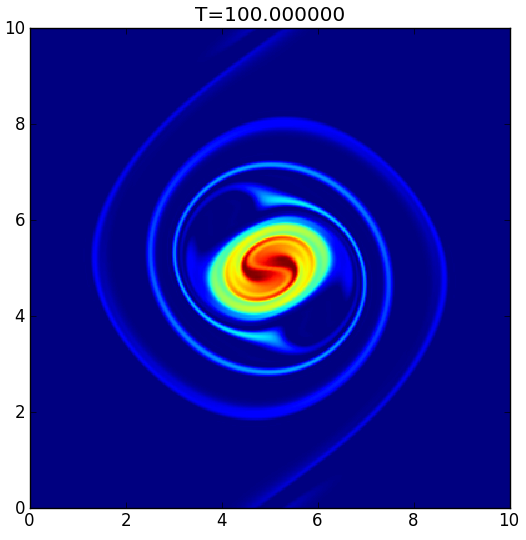
\includegraphics[width=\textwidth]{figures/s139-vortex-waltz_00010.png}
		\end{column}
	\end{columns}

	\begin{block}{Goal}
	      A robust code capable of running very quickly at
	      coarse velocity space resolution while preserving all
	      conservation laws of gyro-fluid/fluid equations and giving
	      fairly good results.
	  \end{block}
\end{frame}

\begin{frame}
\frametitle{Objective}
	Explore basis functions that reduce computational effort, yet retain the formal high-order accuracy for 4-D/5-D gyrokinetic simulations
	\begin{itemize}
		\item 1024 unknowns per element using standard 3rd order element in 5-D
		\item Investigate serendipity basis functions
	\end{itemize}
\end{frame}

\begin{frame}
\frametitle{Hyperbolic PDEs}

\begin{columns}
	\begin{column}{0.5\linewidth}
		\begin{itemize}
			\item Conservation laws \[ \frac{\partial Q}{\partial t} + \nabla \cdot \boldsymbol{F}(Q) = \psi(Q)\]
			\item Wave equations
			\item Euler equations
			\item Navier-Stokes equations
			\item Two-Fluid MHD
			\item Vlasov Equation
			\item Hasegawa-Wakatani equations
			\item Gyrokinetic equations
		\end{itemize}
	\end{column}

	\begin{column}{0.4\linewidth}
		\begin{figure}
			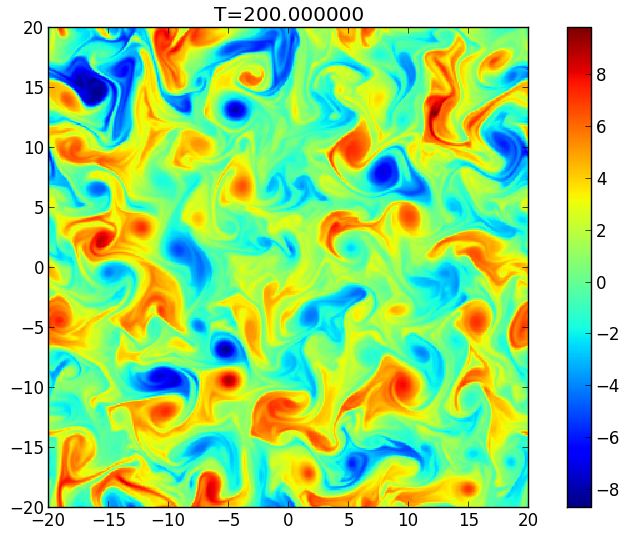
\includegraphics[width=\textwidth]{figures/s217-hw_numDens_00100.png}
		\end{figure}
	\end{column}
\end{columns}
\end{frame}

\section{Summary of Finite Element Methods}
\begin{frame}
	\frametitle{Finite Element Methods}
	\begin{itemize}
		\item Technique for solving systems of PDEs
		\item Example: Consider a differential equation with the exact solution in blue
		\item Seek approximate solution (red) as a sum of piecewise linear functions
	\end{itemize}
	\begin{figure}
	    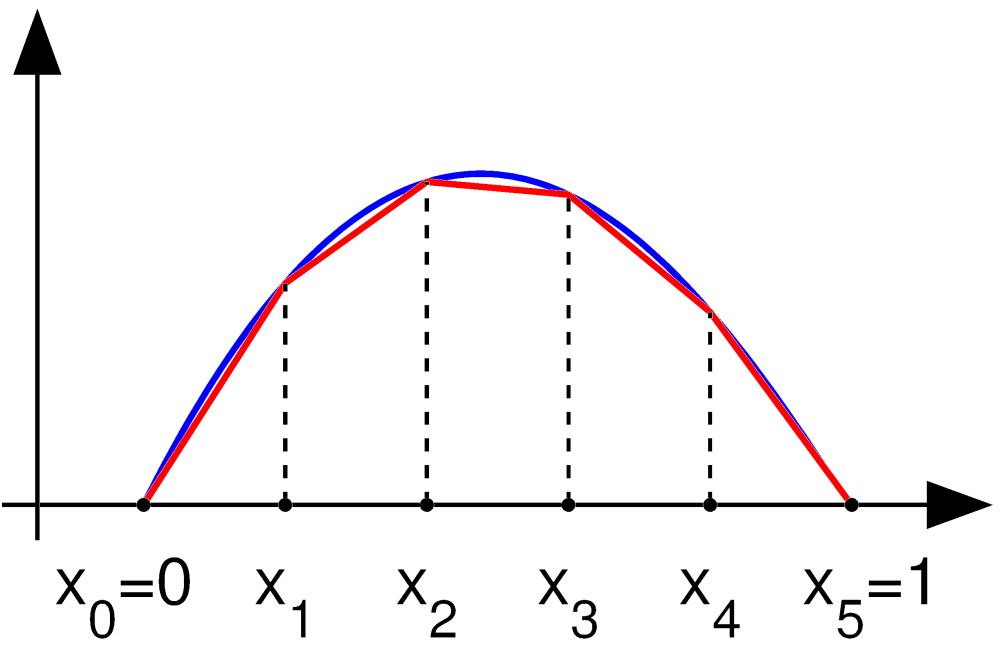
\includegraphics[width=0.50\textwidth]{figures/Finite_element_method_1D_illustration1.png}
	    \let\thefootnote\relax\footnotetext{Image from Wikipedia}
	\end{figure}
\end{frame}

\begin{frame}
\frametitle{Finite Element Methods}
\begin{itemize}
	\item Partition solution domain into elements of simple geometrical shape (mesh)
	\begin{itemize}
		\item Each element contains a number of nodes
	\end{itemize}
	\item Use finite element analysis to find the `optimal' linear combination of \emph{basis functions} for approximate solution
\[u(x) \approx \tilde{u}(x) = \displaystyle\sum_{k=1}^{K}w_k N_k(x), \; N_k(x_j) = \delta_{kj} \]
	\item The $N_k$(x) (blue) are basis functions, $x_k$ are nodes
\begin{figure}
    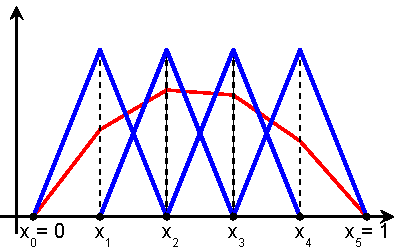
\includegraphics[width=0.40\textwidth]{figures/Finite_element_method_1D_illustration2.pdf}
    \let\thefootnote\relax\footnotetext{Image from Wikipedia}
\end{figure}
\end{itemize}
\end{frame}

\begin{frame}
\frametitle{Finite Element Methods}
\begin{itemize}
	\item Due to basis function properties, approximate solution can be expressed in terms of the \emph{function values} at the nodes
\[u(x) \approx \tilde{u}(x) = \displaystyle\sum_{k=1}^{K}\tilde{u}(x_k)N_k(x), \; N_k(x_j) = \delta_{kj} \]
	\item Solve $K$ algebraic equations to find unknown weights $w_k=\tilde{u}(x_k,t)$
\begin{figure}
    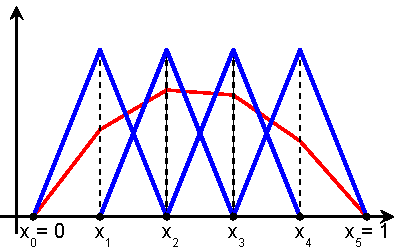
\includegraphics[width=0.40\textwidth]{figures/Finite_element_method_1D_illustration2.pdf}
    \let\thefootnote\relax\footnotetext{Image from Wikipedia}
\end{figure}
\end{itemize}
\end{frame}

\begin{frame}
\frametitle{Finite Element Methods}
\begin{itemize}
	\item \emph{Nodal} basis functions $N_k(x)$ evaluate to 1 at node $x_k$ and 0 at every $x_{j\neq k}$
	\item There is flexibility in choosing basis functions--don't need to use tent functions
	\item Two strategies for increasing accuracy:
	\begin{itemize}
		\item Use smaller elements (more elements to discretize domain)
		\item Use basis functions composed of higher degree polynomials
	\end{itemize}
	\item Cost of using higher-degree basis functions is more degrees of freedom (unknowns) per element
	\begin{itemize}
		\item Use higher-degree basis functions with larger elements?
	\end{itemize}
\end{itemize}
\end{frame}

\begin{frame}
\frametitle{Polynomial Completeness}
\begin{itemize}
\item If basis functions span a complete $N$th degree polynomial and finite elements have length $h$, error behaves as
	\[||u-\tilde{u}|| \leq Ch^{N+1}\]
\item Useful to recall Pascal triangle:
\end{itemize}
\begin{figure}
    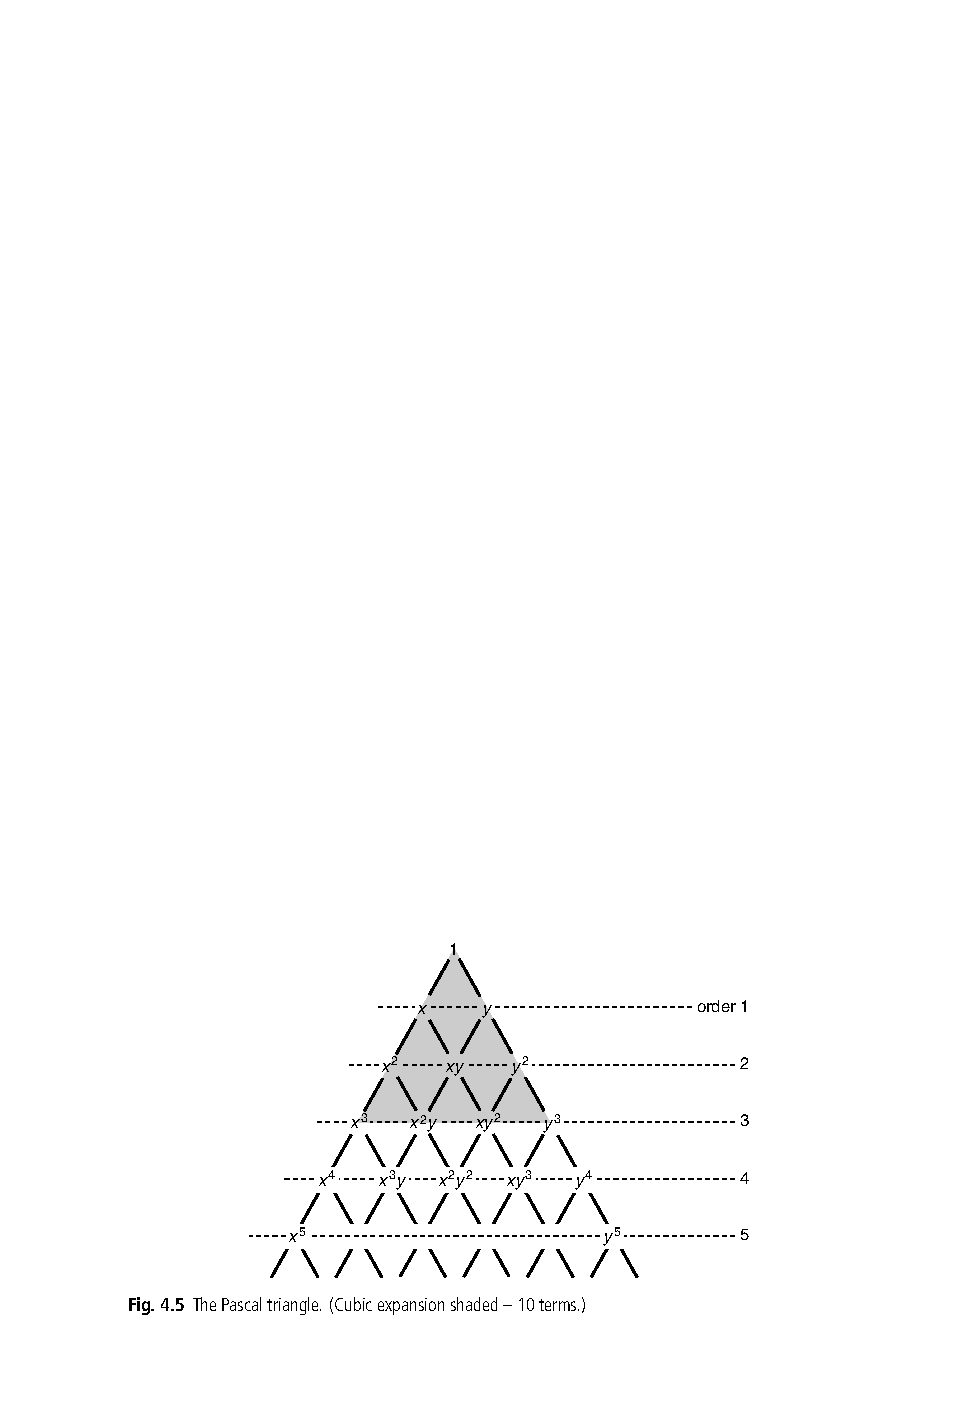
\includegraphics[width=0.6\textwidth]{figures/bookFig2.pdf}
    \let\thefootnote\relax\footnotetext{Image from \emph{The Finite Element Method: Its Basis and Fundamentals}}
\end{figure}
\end{frame}

\begin{frame}
\frametitle{Degrees of Freedom (DOF)}
\begin{itemize}
	\item In the FEM, solution is expressed in terms of a finite number of DOF + basis functions
	\item DOF are the unknown basis function weights, e.g.
\[u(x,t) \approx \tilde{u}(x,t) = \displaystyle\sum_{k=1}^{K}\textcolor{red}{\tilde{u}(x_k,t)}N_k(x) \]
	\item When using \emph{nodal} elements, the DOF are characterized by the value(s) of a function at the nodes of each element
	\begin{itemize}
		\item \# unknowns = \# DOF
		\item Function can be $\tilde{u}$ and/or $\tilde{u}'$
	\end{itemize}
\end{itemize}
\end{frame}

\begin{frame}
\frametitle{Finite Elements in Higher Dimensions}
	\begin{itemize}
		\item 1-D: elements of finite interval
		\item 2-D: elements of finite area (e.g. rectangles, triangles, curvilinear polygons)
		\item 3-D: elements of finite volumes (e.g. cubes, tetrahedra)
		\item All finite elements are transformations of reference elements (e.g. square, triangle, cube)
	\end{itemize}
	\begin{figure}
    	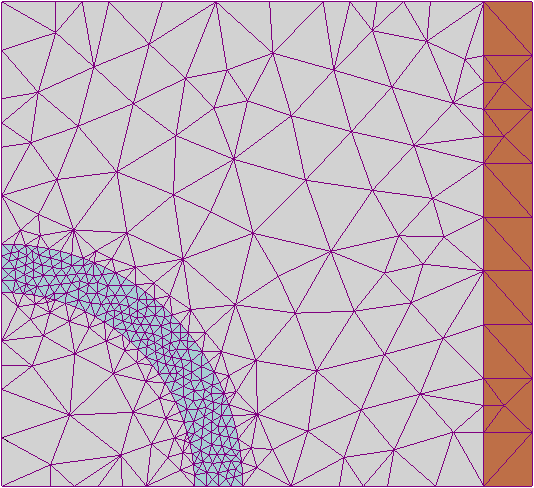
\includegraphics[width=0.3\textwidth]{figures/2d_mesh.png}
    	\caption{Example 2-D FEM mesh using triangles}
    	\let\thefootnote\relax\footnotetext{Image from Wikipedia}
	\end{figure}
\end{frame}

\begin{frame}
\frametitle{Discontinuous Galerkin Background}
	\begin{itemize}
		\item State-of-art for solution of hyperbolic partial differential equations
		\item First introduced by Reed and Hill for steady-state 2-D neutron transport in 1973
		\item Runge-Kutta DG for time-dependent problems by Cockburn and Shu (1998)
		\begin{itemize}
			\item Finite element space discretization, Runge-Kutta time discretization
		\end{itemize}
		\item Widely used in computational fluid dynamics, finding use in more applications (e.g. atmospheric modeling, MHD)
	\end{itemize}
\end{frame}

\begin{frame}{Discontinuous Galerkin Solutions}
  Discontinuous Galerkin schemes use function spaces that allow
  \emph{discontinuities} across cell boundaries.
  \begin{figure}
    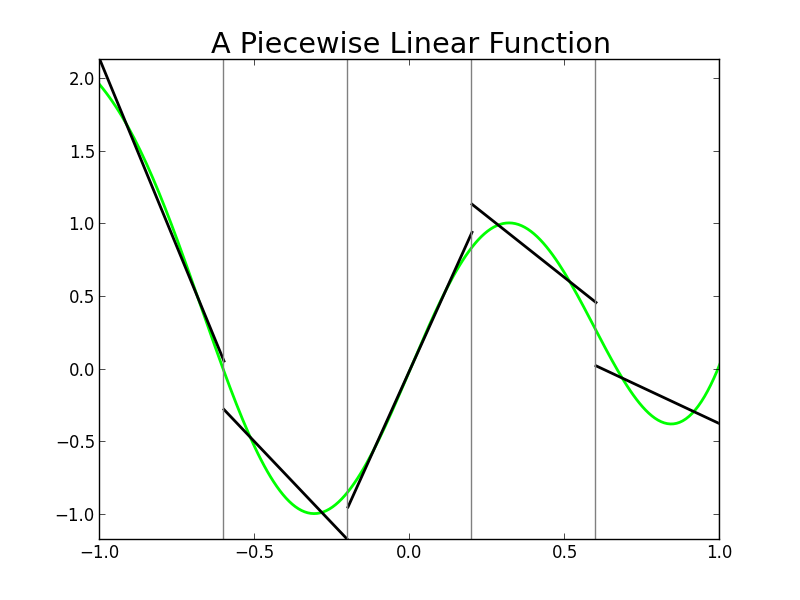
\includegraphics[width=0.5\textwidth]{figures/v1m1.png}
    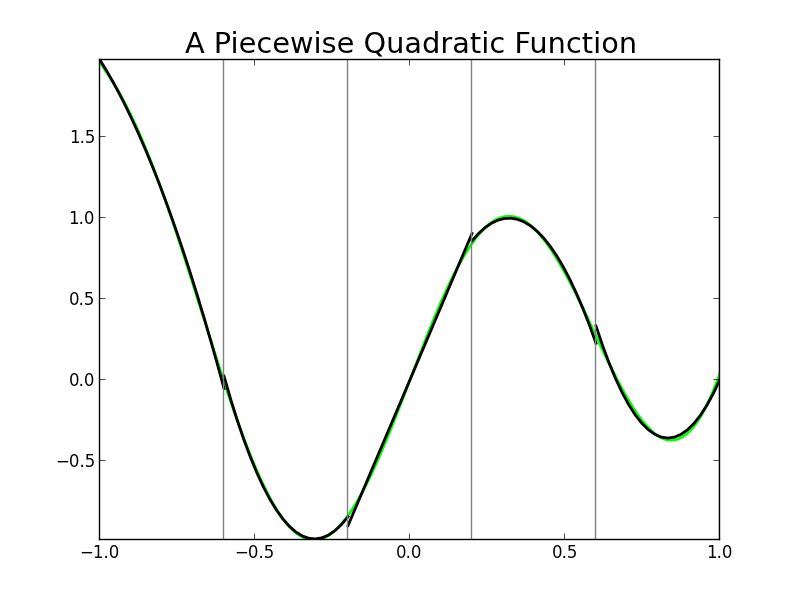
\includegraphics[width=0.5\textwidth]{figures/v2m1.png}
    \caption{The best $L^2$ fit of $x^4+\sin(5x)$ (green) with piecewise
      linear (left) and quadratic (right) basis functions.}
  \end{figure}
\end{frame}

\begin{frame}
\frametitle{Discontinuous Galerkin Features}
	\begin{itemize}
		\item Numerical solution is discontinuous between elements
		\item Hybrid approach: exploit merits of classical finite element and finite volume methods
		\begin{itemize}
			\item FV: slope limiters to control spurious oscillations, locality
			\item FE: high-order accuracy, complex geometries
		\end{itemize}
		\item Information only needs to be shared between neighboring elements--adapts well to massively parallel architectures
	\end{itemize}
	DG combined with FV schemes can lead to best-in-class explicit
  algorithms for \emph{hyperbolic PDEs}.
\end{frame}

\begin{frame}{Finite Elements in DG}
  \begin{itemize}
  	\item Finite elements are non-overlapping
  	\item Basis functions are zero outside the element
  	\item Solution within an element defined only in terms of that element's basis functions and DOF
  	\[u(x,t) \approx \tilde{u}(x,t) = \displaystyle\sum_{k=1}^{K}\tilde{u}(x_k,t)N_k(x) \]
  \end{itemize}
\end{frame}

\section{Finite Element Spaces}
\begin{frame}
\frametitle{Finite Element Spaces}
	\begin{itemize}
		\item Set of all functions that can be written as linear combinations of the basis functions
		\item Specified for each degree and dimension by:
		\begin{enumerate}
			\item Element shape (e.g. triangle, quadrilateral, hexahedron, etc.)
			\item Set of basis functions that span the function space
			\begin{itemize}
				\item \# basis functions per element = \# DOF per element				
				\item (Nodal only): DOF on each face of dimension $d$ (vertex, edge, interior)
			\end{itemize}
		\end{enumerate}
		\item Example finite element spaces:
		\begin{itemize}
		\item Lagrange ($C^0$)
		\item Serendipity ($C^0$)
		\item Hermite Cubic ($C^1$)
		\end{itemize}
	\end{itemize}
\end{frame}

\subsection{Lagrange Family}
\begin{frame}
\frametitle{Lagrange Family}
	\begin{itemize}
		\item Basis functions are tensor products of Lagrange polynomials
		\[ \ell^n_k(x) = \prod^n_{\begin{smallmatrix}i=0 \\ i\neq k\end{smallmatrix}} \frac{x-x_i}{x_k - x_i}, \;
		 N_a(x,y) \equiv l^n_a(x) l^m_a(y) \]
	\end{itemize}
	\begin{figure}
    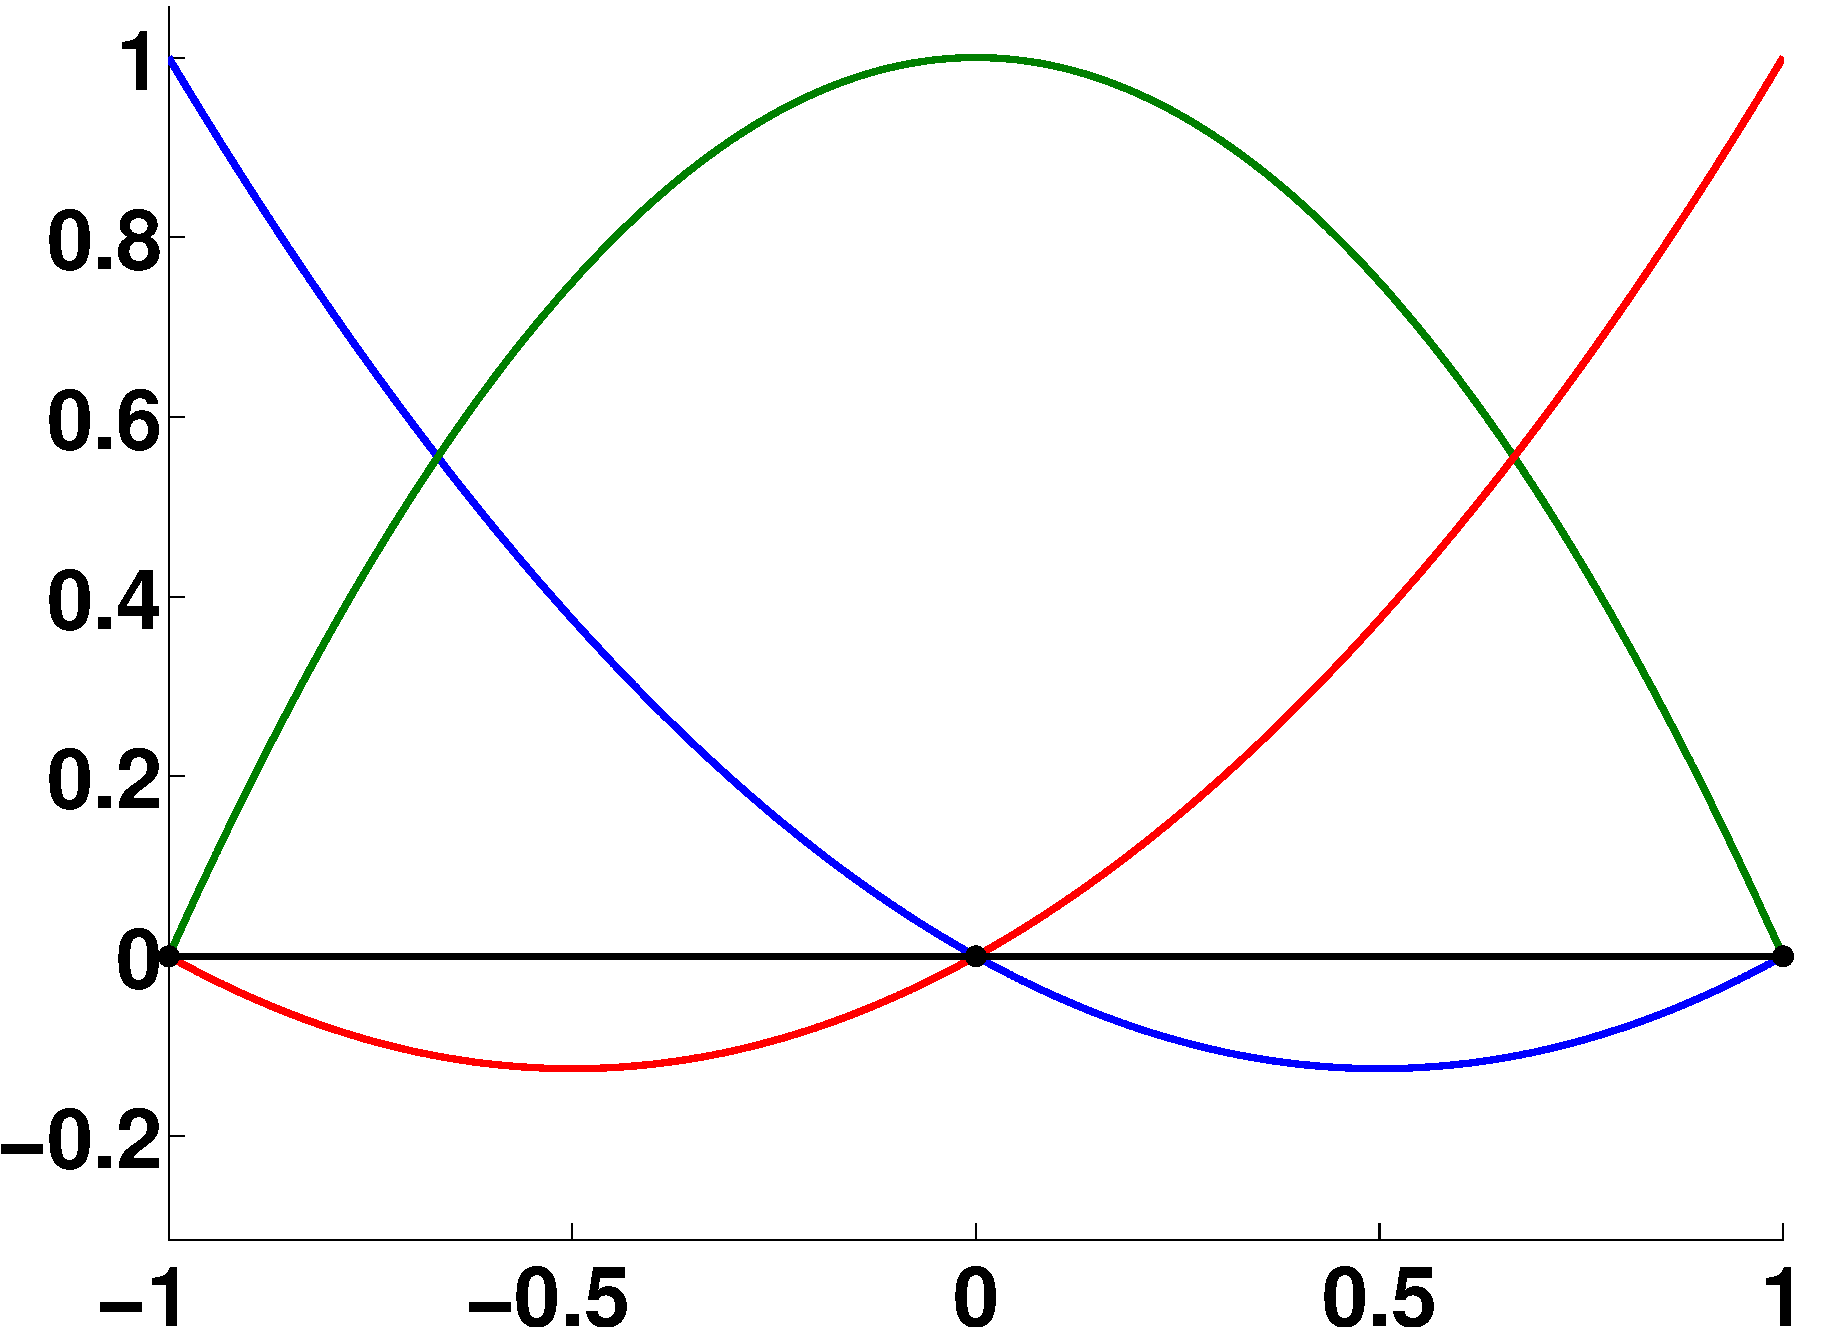
\includegraphics[width=0.4\textwidth]{figures/lagrange3.pdf}
    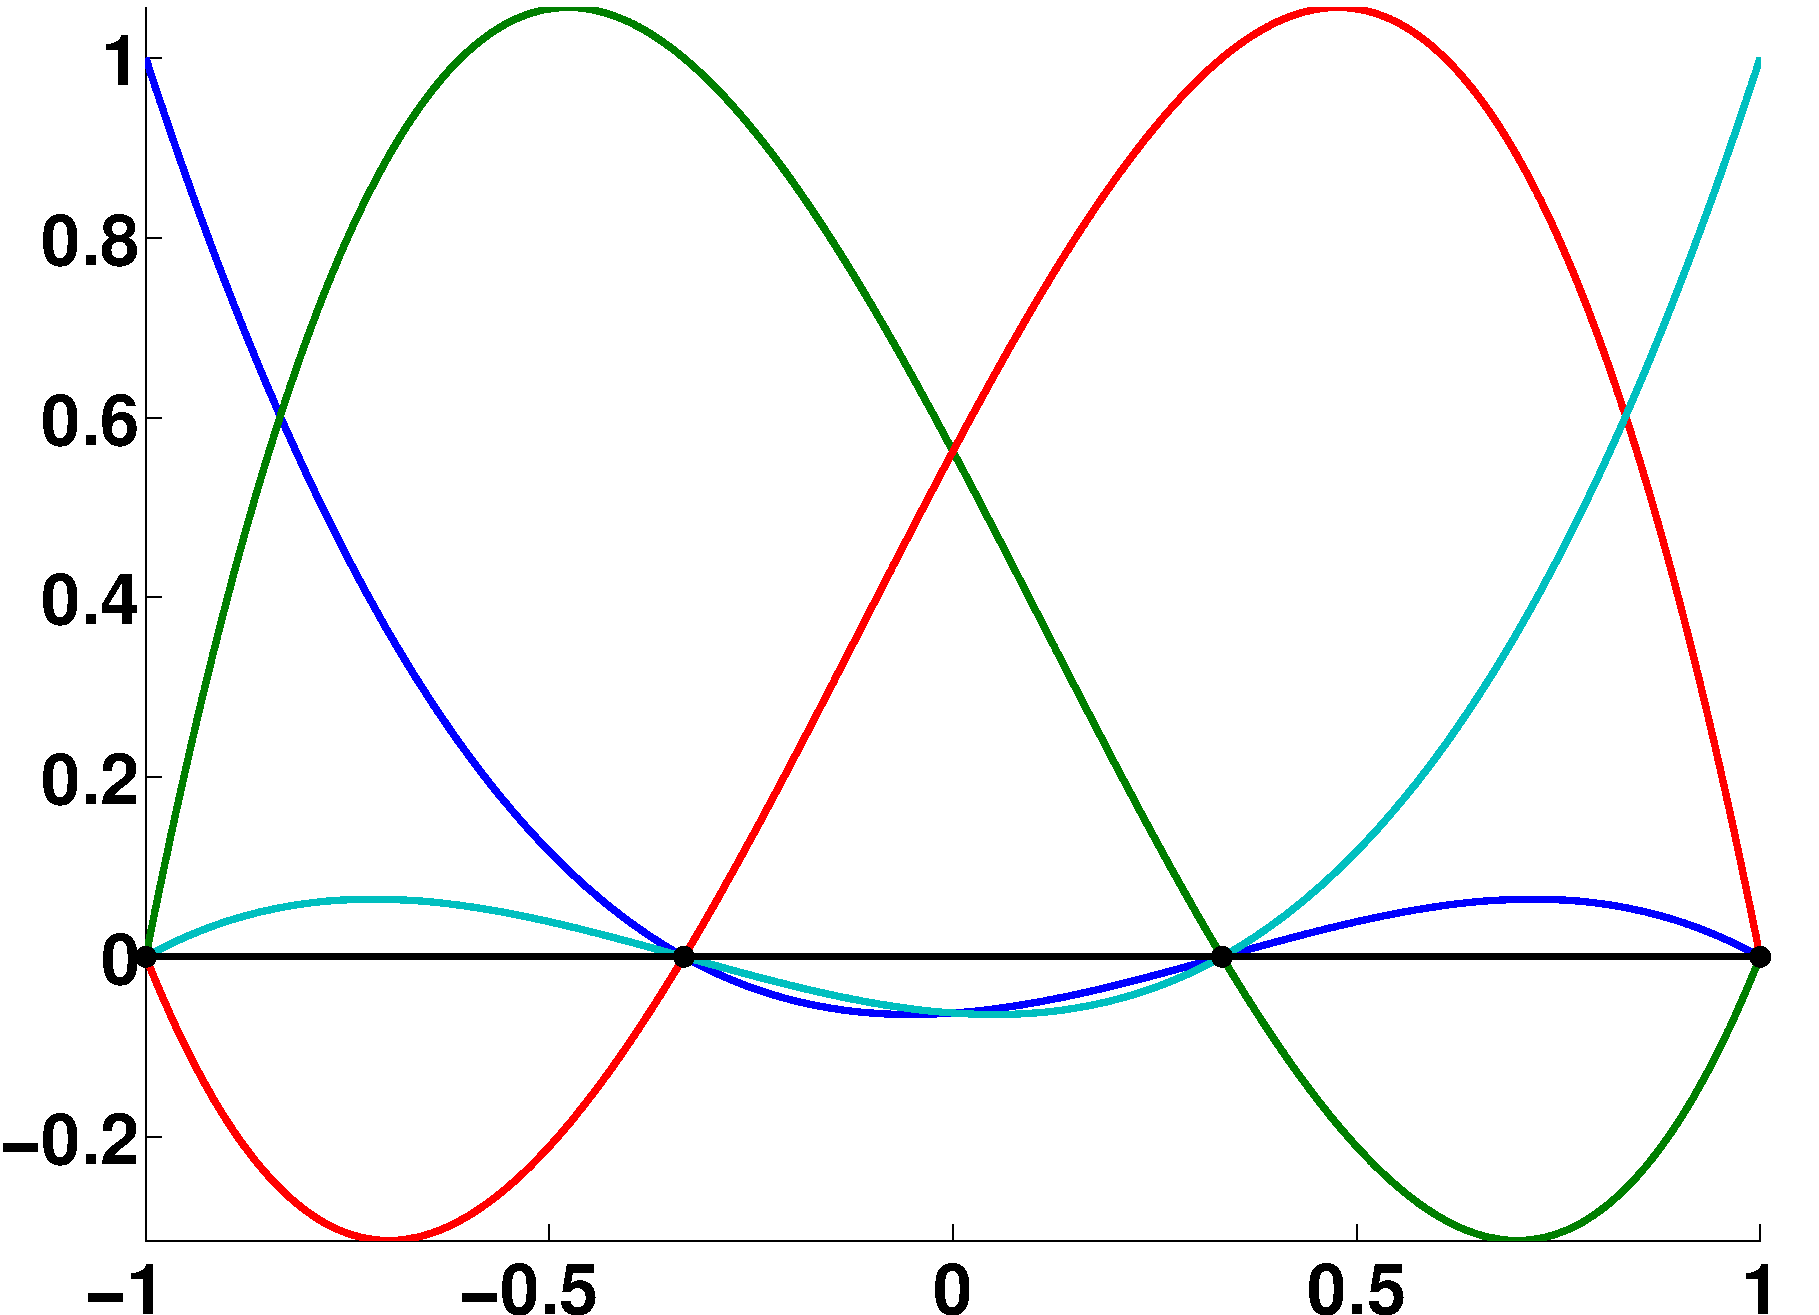
\includegraphics[width=0.4\textwidth]{figures/lagrange4.pdf}
    \caption{Basis functions for 2nd (right) and 3rd (left) order elements.}
  \end{figure}
\end{frame}

\begin{frame}
\frametitle{Lagrange Family}
	\begin{itemize}
		\item Pros: Easy to implement, generalizes to arbitrary dimension and order
		\item Cons: Large number of DOF in higher dimension and order
		\begin{itemize}
			\item In 5-D, need $(3+1)^5=\mathbf{1024}$ DOF per element for 3rd order
		\end{itemize}
		\item Large number of terms above those needed for complete expansion present!
	\end{itemize}
	\begin{figure}
	    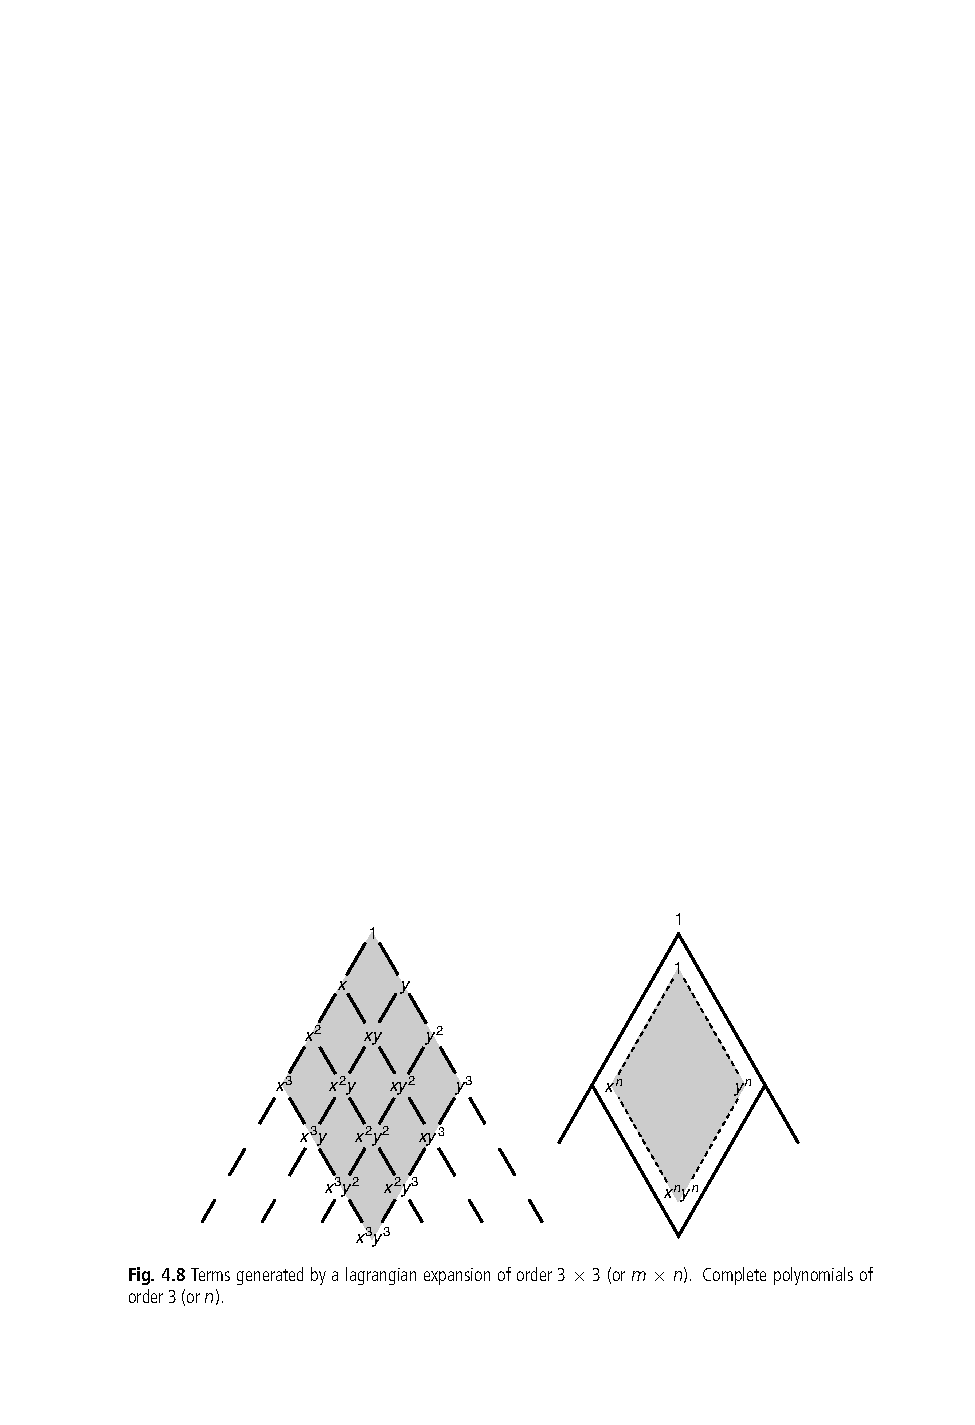
\includegraphics[width=0.6\textwidth]{figures/bookFig3.pdf}
	    \let\thefootnote\relax\footnotetext{Image from \emph{The Finite Element Method: Its Basis and Fundamentals}}
	\end{figure}
\end{frame}

\subsection{Serendipity Family}
\begin{frame}
\frametitle{Serendipity Family}
	\begin{itemize}
		\item Basis functions originally derived by inspection (`serendipity')
		\item Fewer interior nodes compared to Lagrange element of same order
		\begin{itemize}
			\item Fewer DOF per element
			\item Smaller dimension function space
		\end{itemize}
		\item Expect lower accuracy, but faster than Lagrange elements of the same order
	\end{itemize}
	\begin{block}{Key Question}
		Can serendipity elements deliver the same error at a lower computational cost (by choice of element size and order)?
	\end{block}
\end{frame}

\begin{frame}
\frametitle{Lagrange and Serendipity Compared in 2-D}
	\begin{figure}
		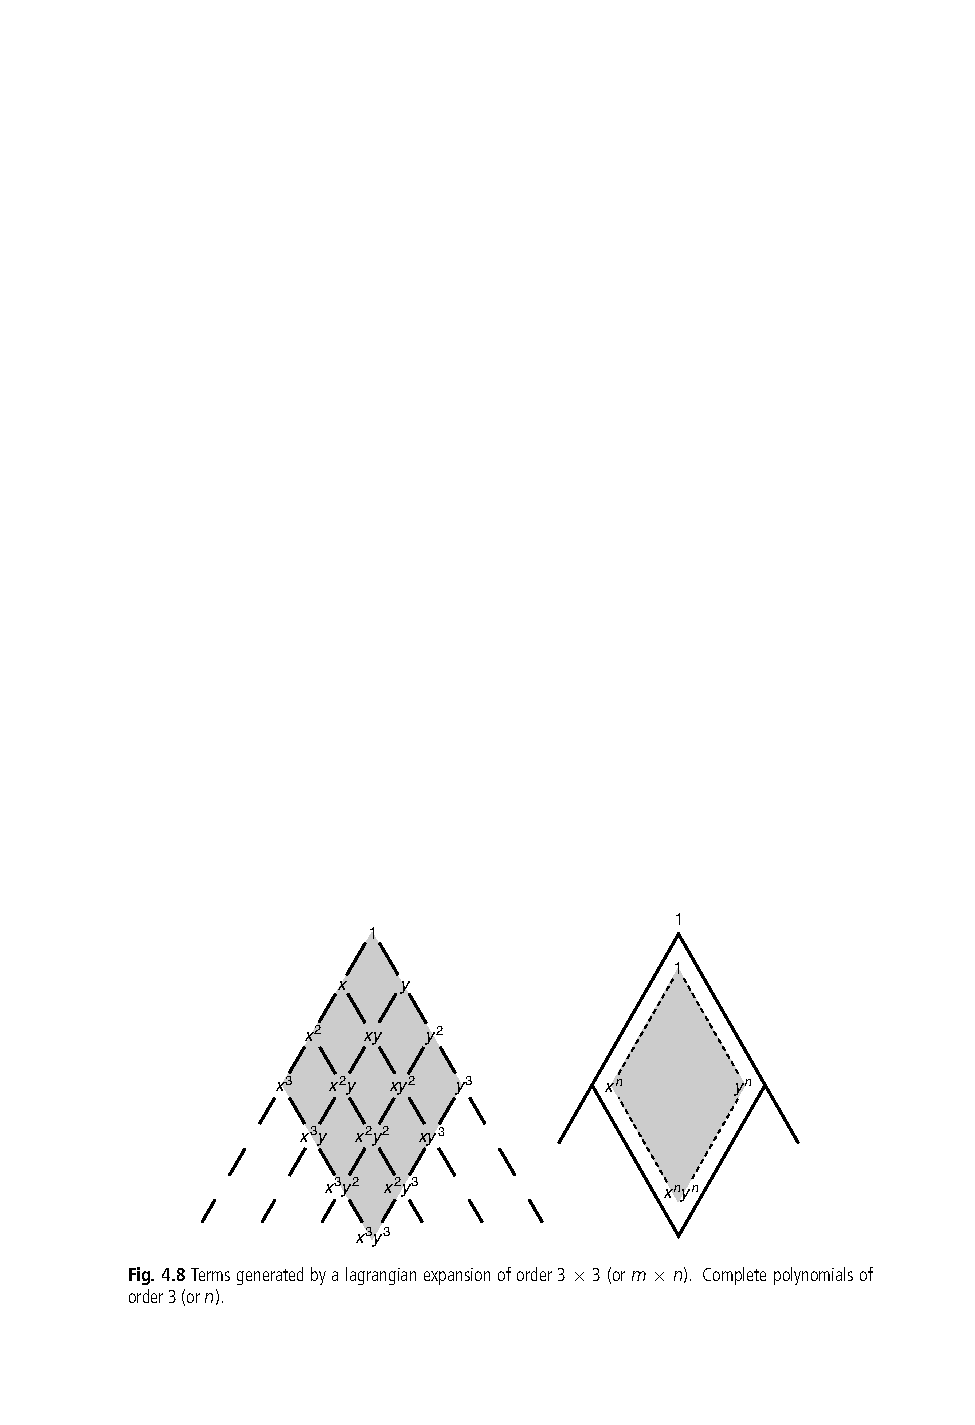
\includegraphics[width=0.6\textwidth]{figures/bookFig3.pdf}\\
	    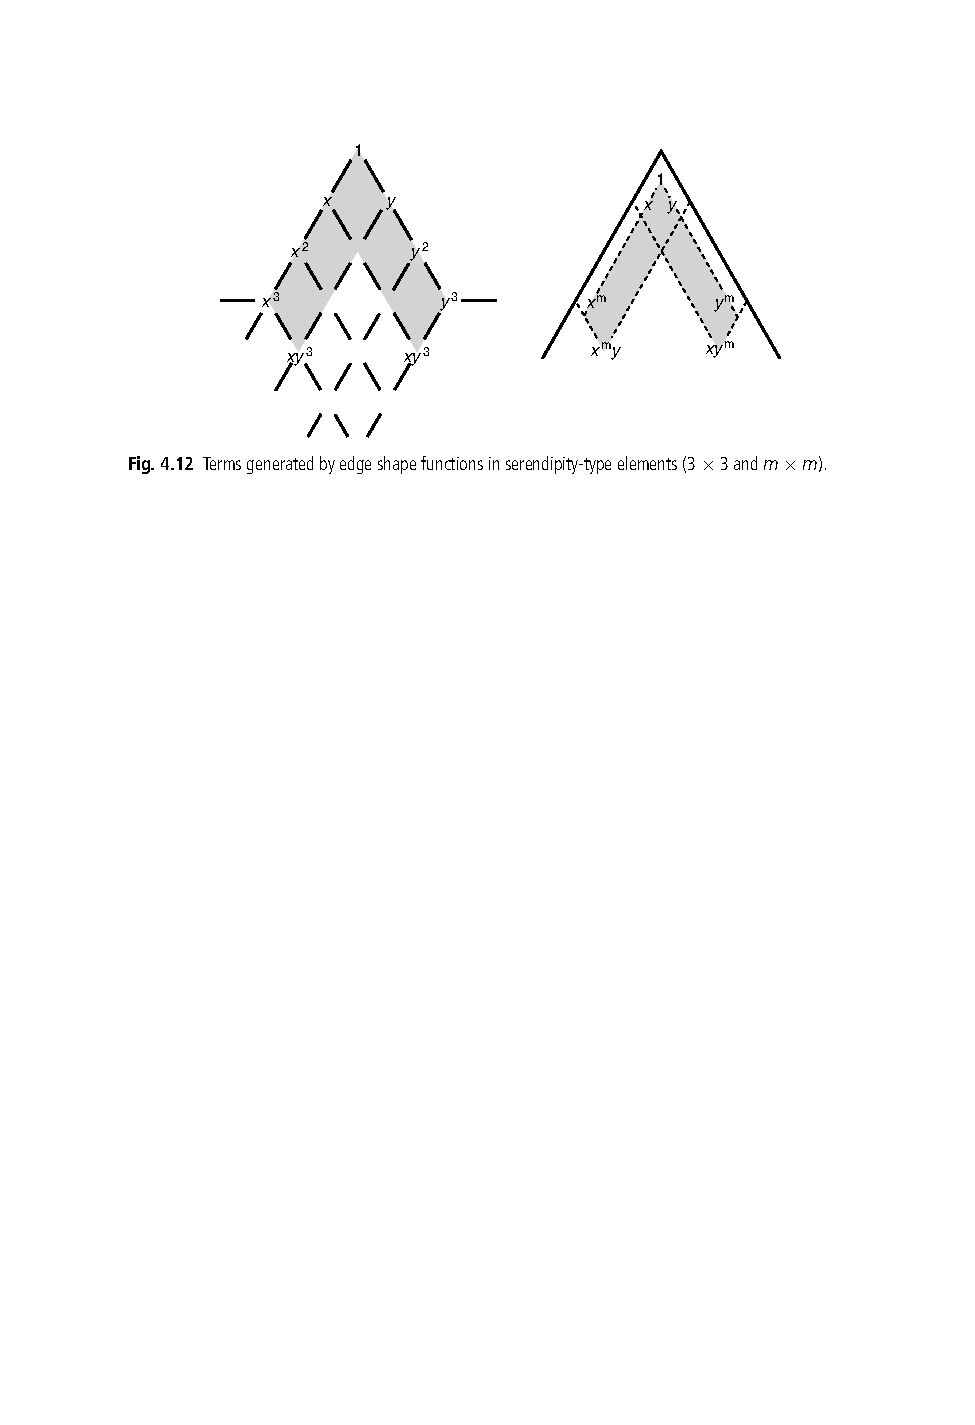
\includegraphics[width=0.6\textwidth]{figures/bookFig4.pdf}
	    \let\thefootnote\relax\footnotetext{Image from \emph{The Finite Element Method: Its Basis and Fundamentals}}
	\end{figure}
\end{frame}

\begin{frame}
\frametitle{Lagrange and Serendipity Compared in 2-D}
	\begin{figure}
	    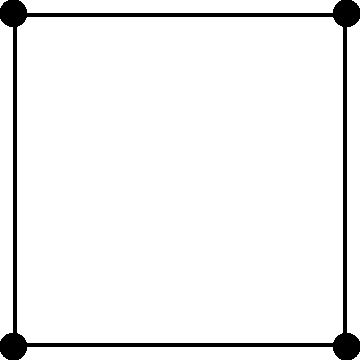
\includegraphics[width=0.20\textwidth]{figures/r1d2.pdf}
	    \hfill
	    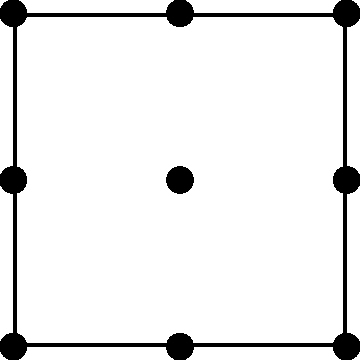
\includegraphics[width=0.20\textwidth]{figures/r2d2_lagrange.pdf}
	    \hfill
	    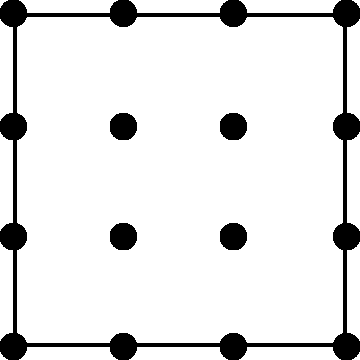
\includegraphics[width=0.20\textwidth]{figures/r3d2_lagrange.pdf}
	    \hfill
	    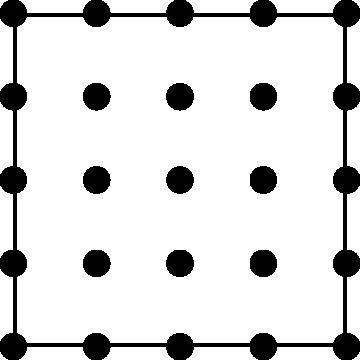
\includegraphics[width=0.20\textwidth]{figures/r4d2_lagrange.pdf}
	    \caption{Node placement of 1st to 4th order Lagrange elements.}
	\end{figure}

	\begin{figure}
	    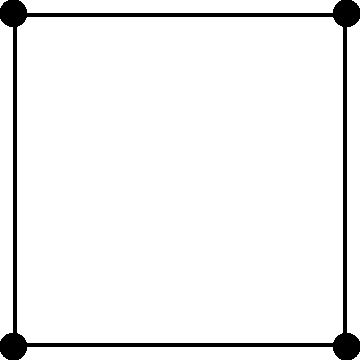
\includegraphics[width=0.20\textwidth]{figures/r1d2.pdf}
	    \hfill
	    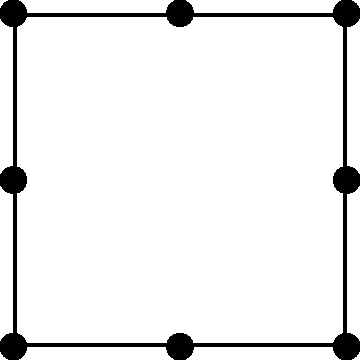
\includegraphics[width=0.20\textwidth]{figures/r2d2.pdf}
	    \hfill
	    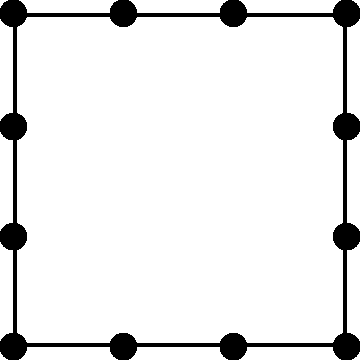
\includegraphics[width=0.20\textwidth]{figures/r3d2.pdf}
	    \hfill
	    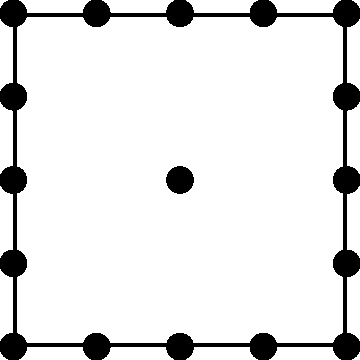
\includegraphics[width=0.20\textwidth]{figures/r4d2.pdf}
	    \caption{Node placement of 1st to 4th order Serendipity elements.}
	\end{figure}
\end{frame}

\begin{frame}
\frametitle{Larger savings in higher dimensions and order}
\begin{columns}
	\begin{column}{0.5\linewidth}
		\begin{tabular}{c|cc}
			\multicolumn{3}{c}{{\bf Three Dimensions}} \\
			\hline
			Order & Lagrange & Serendipity \\
			\hline
			1 & 8 & 8 \\
			2 & 27 & 20 \\
			3 & 64 & 32 \\
			4 & 125 & 50
		\end{tabular}
		\begin{tabular}{c|cc}
			\multicolumn{3}{c}{{\bf Five Dimensions}} \\
			\hline
			Order & Lagrange & Serendipity \\
			\hline
			1 & 32 & 32 \\
			2 & 243 & 112 \\
			3 & 1024 & 192 \\
			4 & 3125 & 352
		\end{tabular}
	\end{column}

	\begin{column}{0.4\linewidth}
		\begin{figure}
			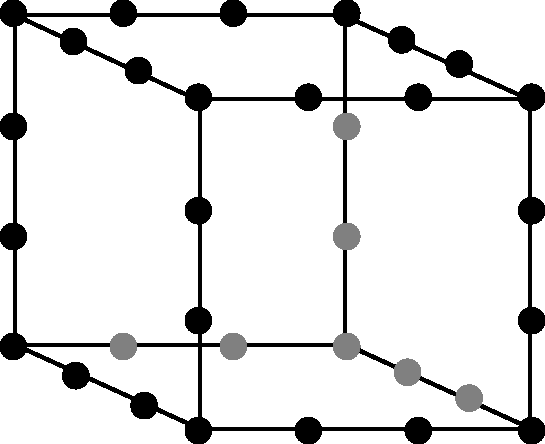
\includegraphics[width=.8\textwidth]{figures/r3d3.pdf}
		    \caption{3rd order Serendipity element in 3-D}
		\end{figure}
	\end{column}
\end{columns}
\end{frame}


\begin{frame}
\frametitle{Serendipity Family Definition}
	\begin{itemize}
		\item Typically used with low order (r$<$3) in 2-D and to a lesser extent in 3-D
		\item Pattern for progression to higher orders, higher dimensions not evident (`serendipity')
		\item Simple and new dimension-independent definition given by Arnold\footfullcite{serendipity} for serendipity elements
	\begin{definition}
The serendipity space $\mathcal{S}_r(I^n)$ is the space of all polynomials in $n$ variables with superlinear degree (total degree with respect to variables entering at least quadratically) at most $r$.
\end{definition}
\end{itemize}
\end{frame}

\begin{frame}
\frametitle{Example: Degree 3 Polynomial Spaces (2-D)}
	{\footnotesize
		\begin{align*}
		\mathcal{P}_r(I^n) :=& \text{span} \{ \text{monomials in n variables with degree} \leq r \}\\
		\mathcal{S}_r(I^n) :=& \text{span} \{ \text{monomials in n variables with superlinear degree} \leq r \} \\
		\mathcal{Q}_r(I^n) :=& \text{span} \{ \text{monomials in n variables with each variable degree} \leq r \}
		\end{align*}
	}%

	\begin{align*}
	\mathcal{P}_3(I^2) =& \; \text{span} \{ 1,x,y,x^2,y^2,xy,x^3,y^3,x^2y,xy^2 \}\\
	\mathcal{S}_3(I^2) =& \; \mathcal{P}_3(I^2) \cup \text{span} \{ x^3y,xy^3 \} \\
	\mathcal{Q}_3(I^2) =& \; \mathcal{S}_3(I^2) \cup \text{span} \{ x^2y^2,x^3y^2,x^2y^3,x^3y^3 \} \\
	\end{align*}
	
	\begin{itemize}
		\item Note that $\mathcal{P}_r(I^n) \subset \mathcal{S}_r(I^n) \subset \mathcal{Q}_r(I^n)$
	\end{itemize}
\end{frame}

\begin{frame}
\frametitle{Example: $\mathcal{S}_2(I^2)$ Basis Functions}
\begin{columns}
	\begin{column}{0.6\linewidth}
		
		$\left(\renewcommand{\arraystretch}{1.5}\begin{array}{c} N_0\\N_1\\N_2\\N_3\\N_4\\N_5\\N_6\\N_7\end{array}\right)=\left(\renewcommand{\arraystretch}{1.5}\begin{array}{c} -\frac{\left(x - 1\right)\, \left(y - 1\right)\, \left(x + y + 1\right)}{4}\\ \frac{\left(x^2 - 1\right)\, \left(y - 1\right)}{2}\\ \frac{\left(x + 1\right)\, \left(y - 1\right)\, \left(y - x + 1\right)}{4}\\ -\frac{\left(y^2 - 1\right)\, \left(x + 1\right)}{2}\\ \frac{\left(x + 1\right)\, \left(y + 1\right)\, \left(x + y - 1\right)}{4}\\ -\frac{\left(x^2 - 1\right)\, \left(y + 1\right)}{2}\\ \frac{\left(x - 1\right)\, \left(y + 1\right)\, \left(x - y + 1\right)}{4}\\ \frac{\left(y^2 - 1\right)\, \left(x - 1\right)}{2} \end{array}\right)
$

	\end{column}

	\begin{column}{0.4\linewidth}
		\begin{figure}
			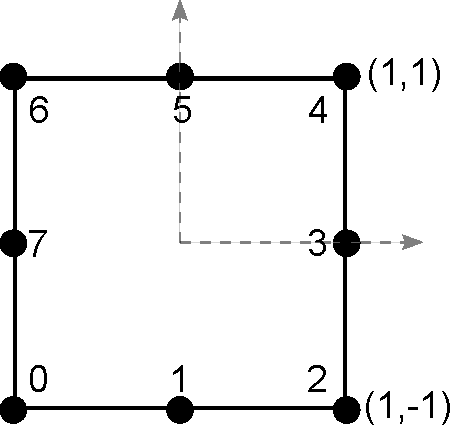
\includegraphics[width=.8\textwidth]{figures/r2d2_labels_2.pdf}
			\caption{$\mathcal{S}_2(I^2)$ element centered at origin}
		\end{figure}
	\end{column}
\end{columns}
\end{frame}

\begin{frame}
\frametitle{Generating Serendipity Basis Functions}
	\begin{enumerate}
		\item Given an order and dimension, determine the monomials $v_k$ that span the serendipity space
		\item Determine location of nodes $\mathbf{x_k}$ on reference element
		\item Set up matrix equation for basis functions
		\[N_j (\mathbf{x}) = \displaystyle\sum\limits_{k} c_j^{(k)}v_k(\mathbf{x}) \]
		\[N_j (\mathbf{x_k}) = \delta_{kj} \]
		\item Solve system for weights $c_j^{(k)}$ by a matrix inversion
		\item Map reference space basis functions to physical space
	\end{enumerate}
\end{frame}

\section{Results}

\begin{frame}
\frametitle{3-D Gaussian Pulse Advection}
\begin{itemize}
	\item Advection at constant speed in 3-D \[\frac{\partial f}{\partial t} +\nabla\cdot\left( f {\bold u}\right) = 0\]
	\item Solution is given by \[f({\bold x},t) = f_0({\bold x}-{\bold u}t)\]
	\item Periodic boundary conditions
	\item Design simulation to end when pulse has completed one period of its motion
	\item Compute error \emph{per node} by summing over all nodes in domain: \[E = \displaystyle\sum\limits_{k}^{N_{nodes}}\frac{|u(t_f,\vec{x_k})-u(t_0,\vec{x_k})|}{N_{nodes}}\]
\end{itemize}
\end{frame}

\begin{frame}
  \begin{figure}
    \includemovie[attach=false,
    poster=movies/pulse.png,
	repeat]{0.5\linewidth}{0.462\linewidth}{figures/movies.mpeg}
    \caption{[Movie] Gaussian pulse advection problem using 3rd order serendipity elements on a $16\times 16\times 16$ grid.}
  \end{figure}
\end{frame}

\begin{frame}
\frametitle{Convergence Study}
	\begin{itemize}
		\item Order of serendipity element and total number of elements varied ($n\times n\times n$ for $n=4,8,16,32$)
		\item Since error $E$ scales as $O(h^c)$ with element size $h$, plot $\log E$ vs. $\log h$ and find slope of best-fit line
	\end{itemize}
	\begin{center}
	\begin{tabular}{c|c|c}
		Order of Element & Order of Scheme (S) & Order of Scheme (L) \\
		\hline
		1 & 2.09 & 2.09 \\
		2 & 3.30 & 3.20 \\
		3 & 3.85 & 4.31\\
		4 & 4.40 & 5.13
	\end{tabular}
	\end{center}
\end{frame}

\begin{frame}
\frametitle{Error vs. Element Size}
\begin{figure}
    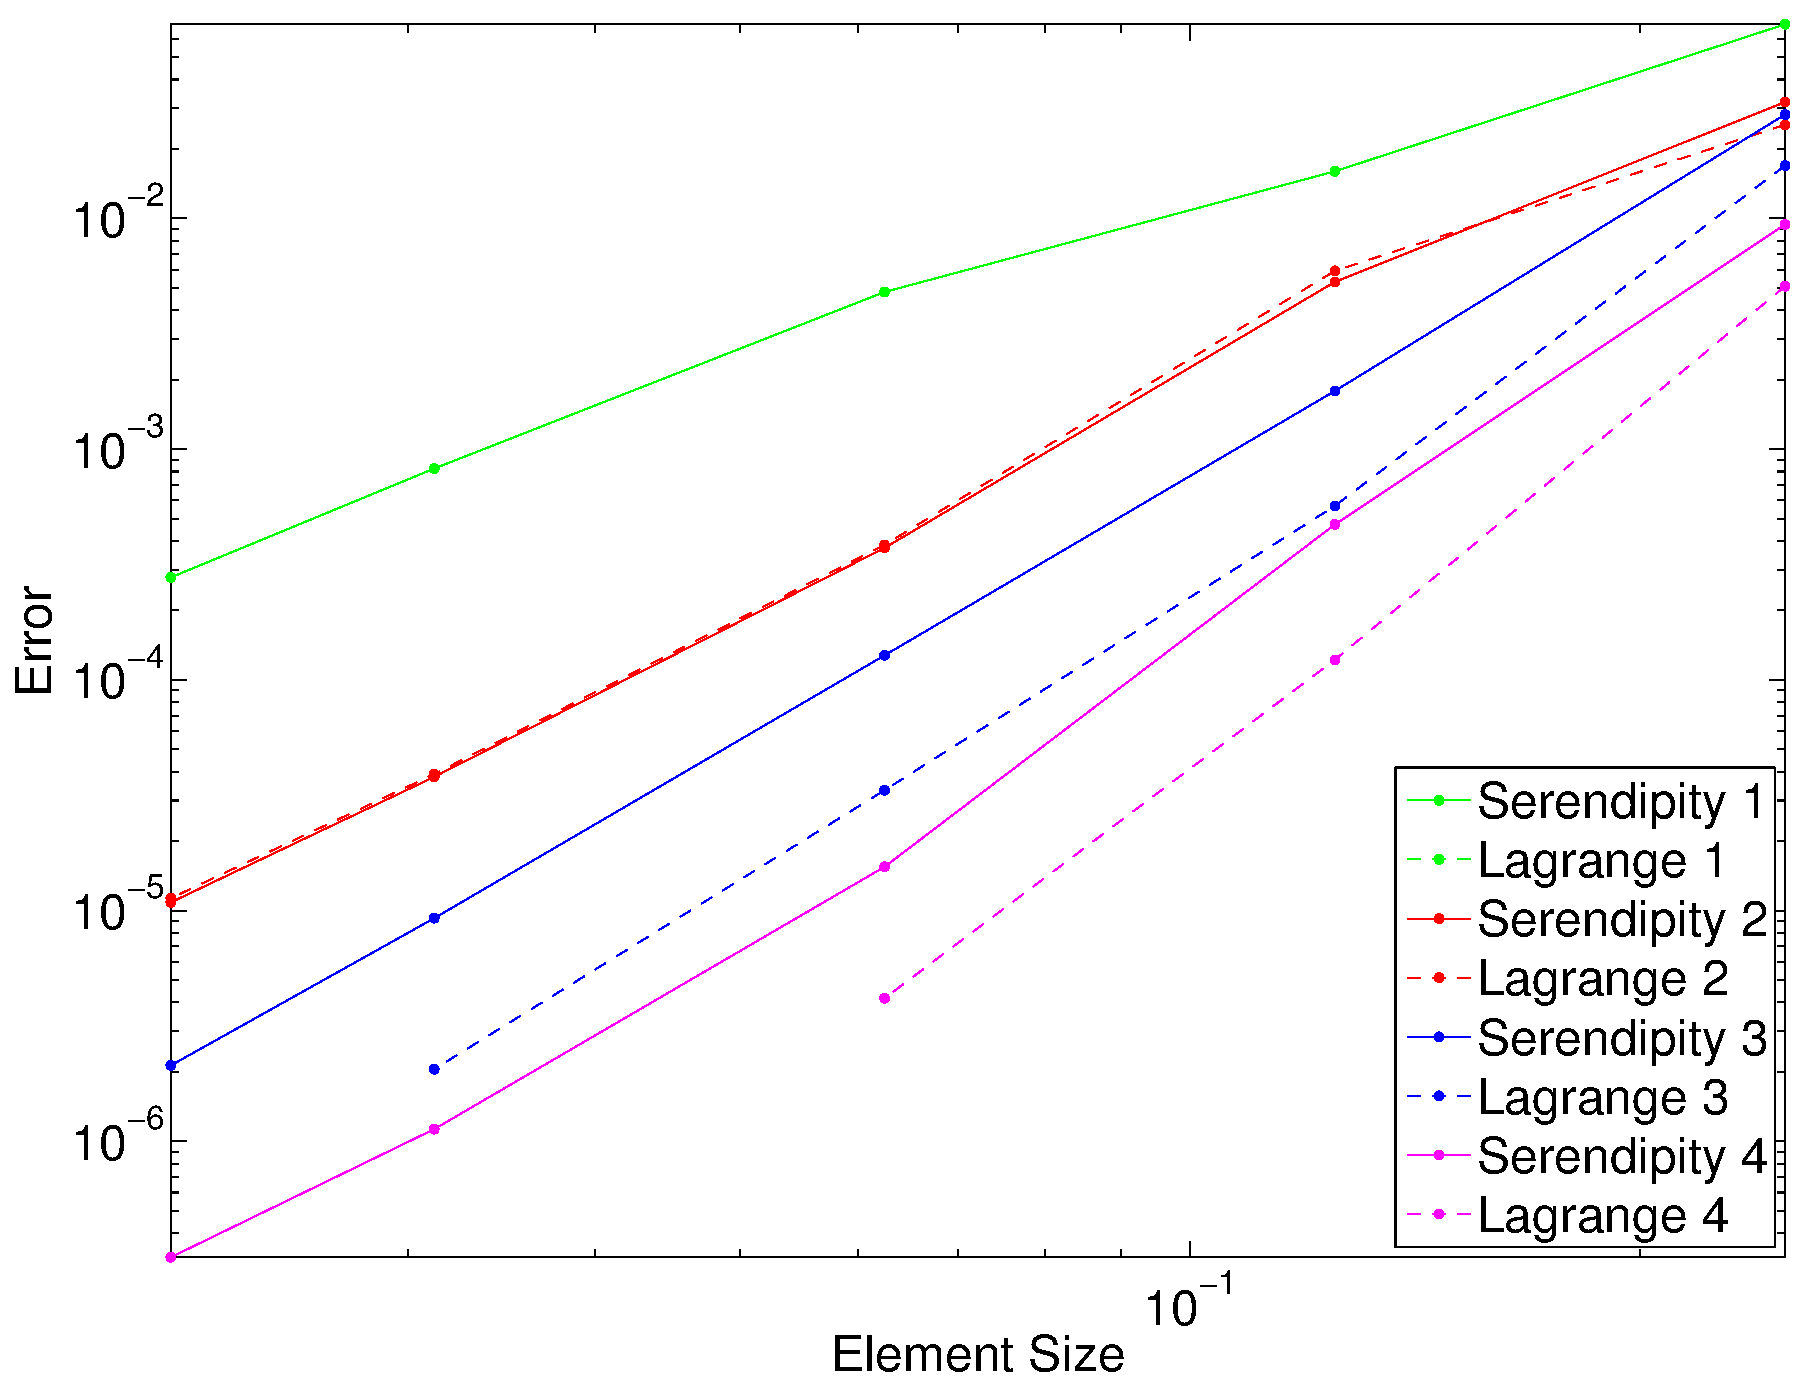
\includegraphics[width=0.8\textwidth]{figures/serendipityError.pdf}
\end{figure}
\end{frame}

\begin{frame}
\frametitle{Computation Time}
	\begin{itemize}
		\item Execution time results for a $32\times 32 \times 32$ element grid:
		\begin{tabular}{c|c|c|c}
			Order of Element & Serendipity & Lagrange & Ratio \\
			\hline
			1 & 73.2 s & 73.2 s & 1.00 \\
			2 & 220 s & 663 s & 0.331 \\
			3 & 654 s & 5350 s & 0.122\\
		\end{tabular}
		\item DOF per element comparison:
		\begin{tabular}{c|c|c|c}
			Order of Element & Serendipity & Lagrange & Ratio \\
			\hline
			1 & 8   & 8  & 1.00 \\
			2 & 20 & 27 & 0.741 \\
			3 & 32 & 64 & 0.500 \\
		\end{tabular}
	\end{itemize}
	Additional savings due to larger permissible time step for serendipity elements
\end{frame}

\begin{frame}
\frametitle{Error vs. Computation Time}
	\begin{figure}
   		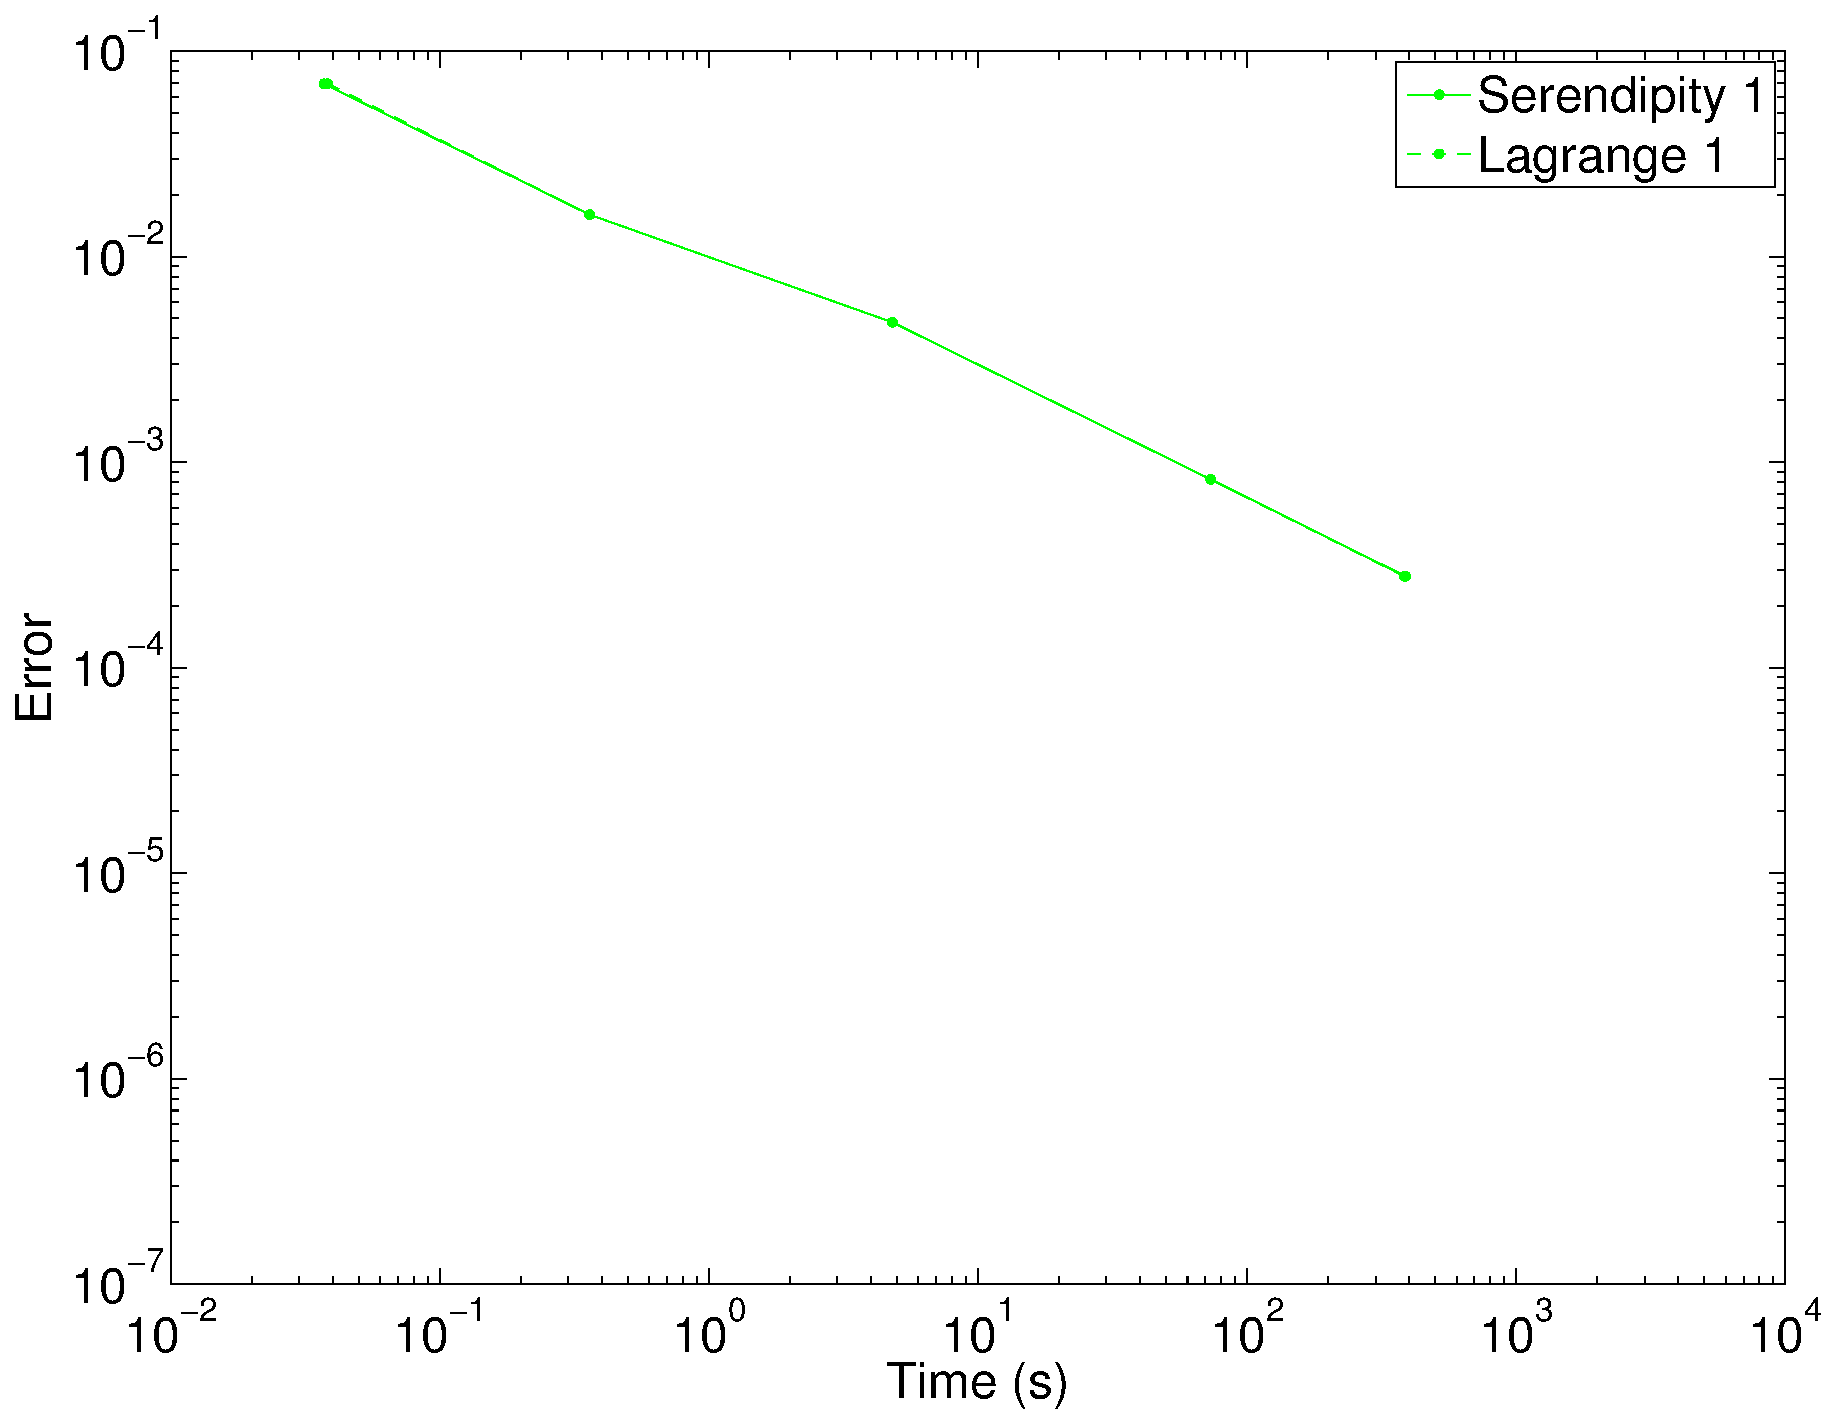
\includegraphics[width=0.8\textwidth]{figures/serendipityConvergence1.pdf}
	\end{figure}
\end{frame}

\begin{frame}
\frametitle{Error vs. Computation Time}
	\begin{figure}
   		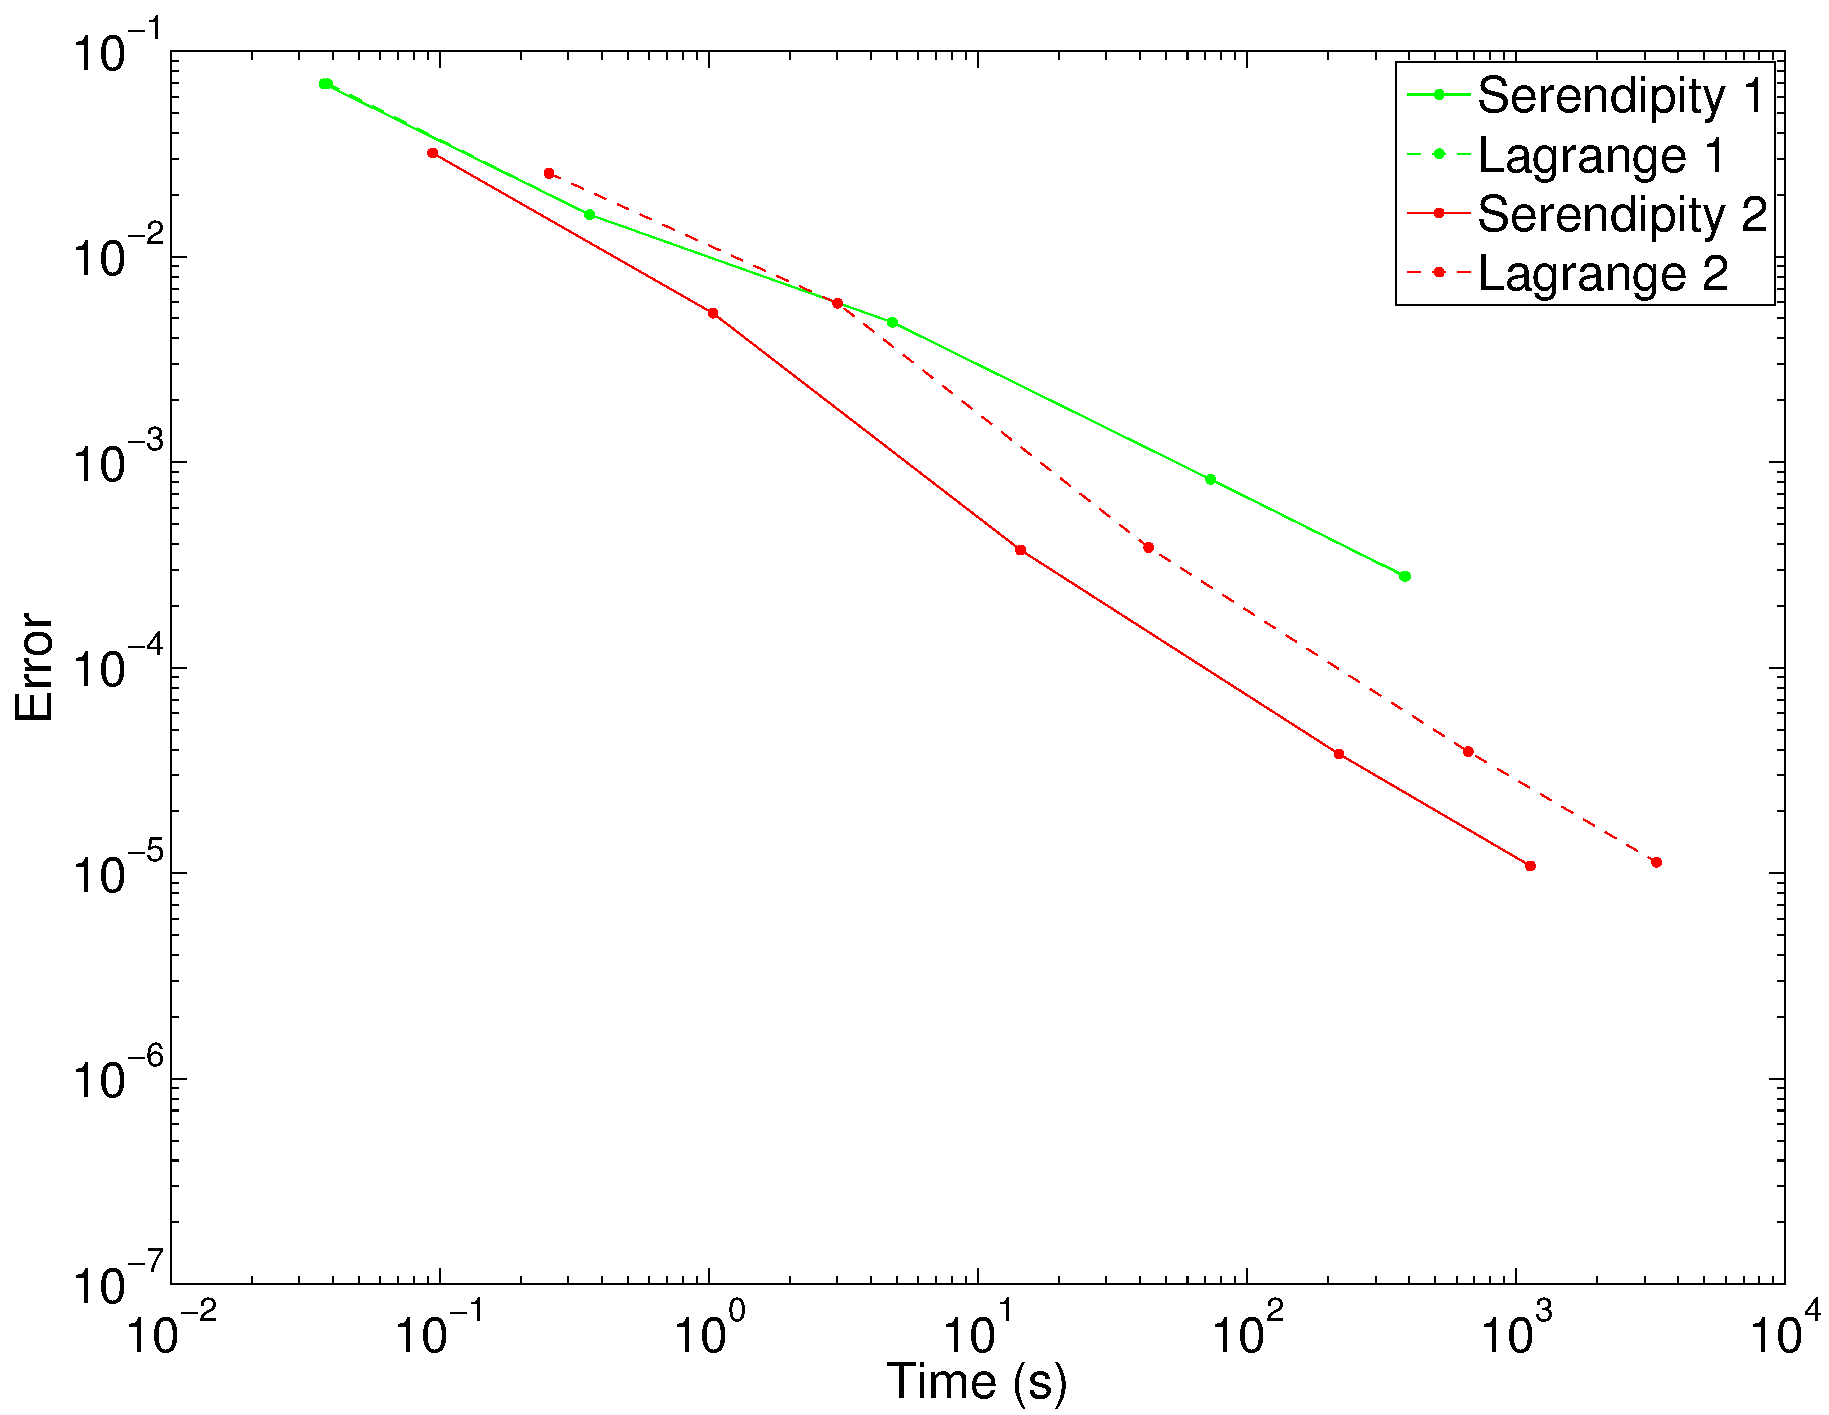
\includegraphics[width=0.8\textwidth]{figures/serendipityConvergence2.pdf}
	\end{figure}
\end{frame}

\begin{frame}
\frametitle{Error vs. Computation Time}
	\begin{figure}
   		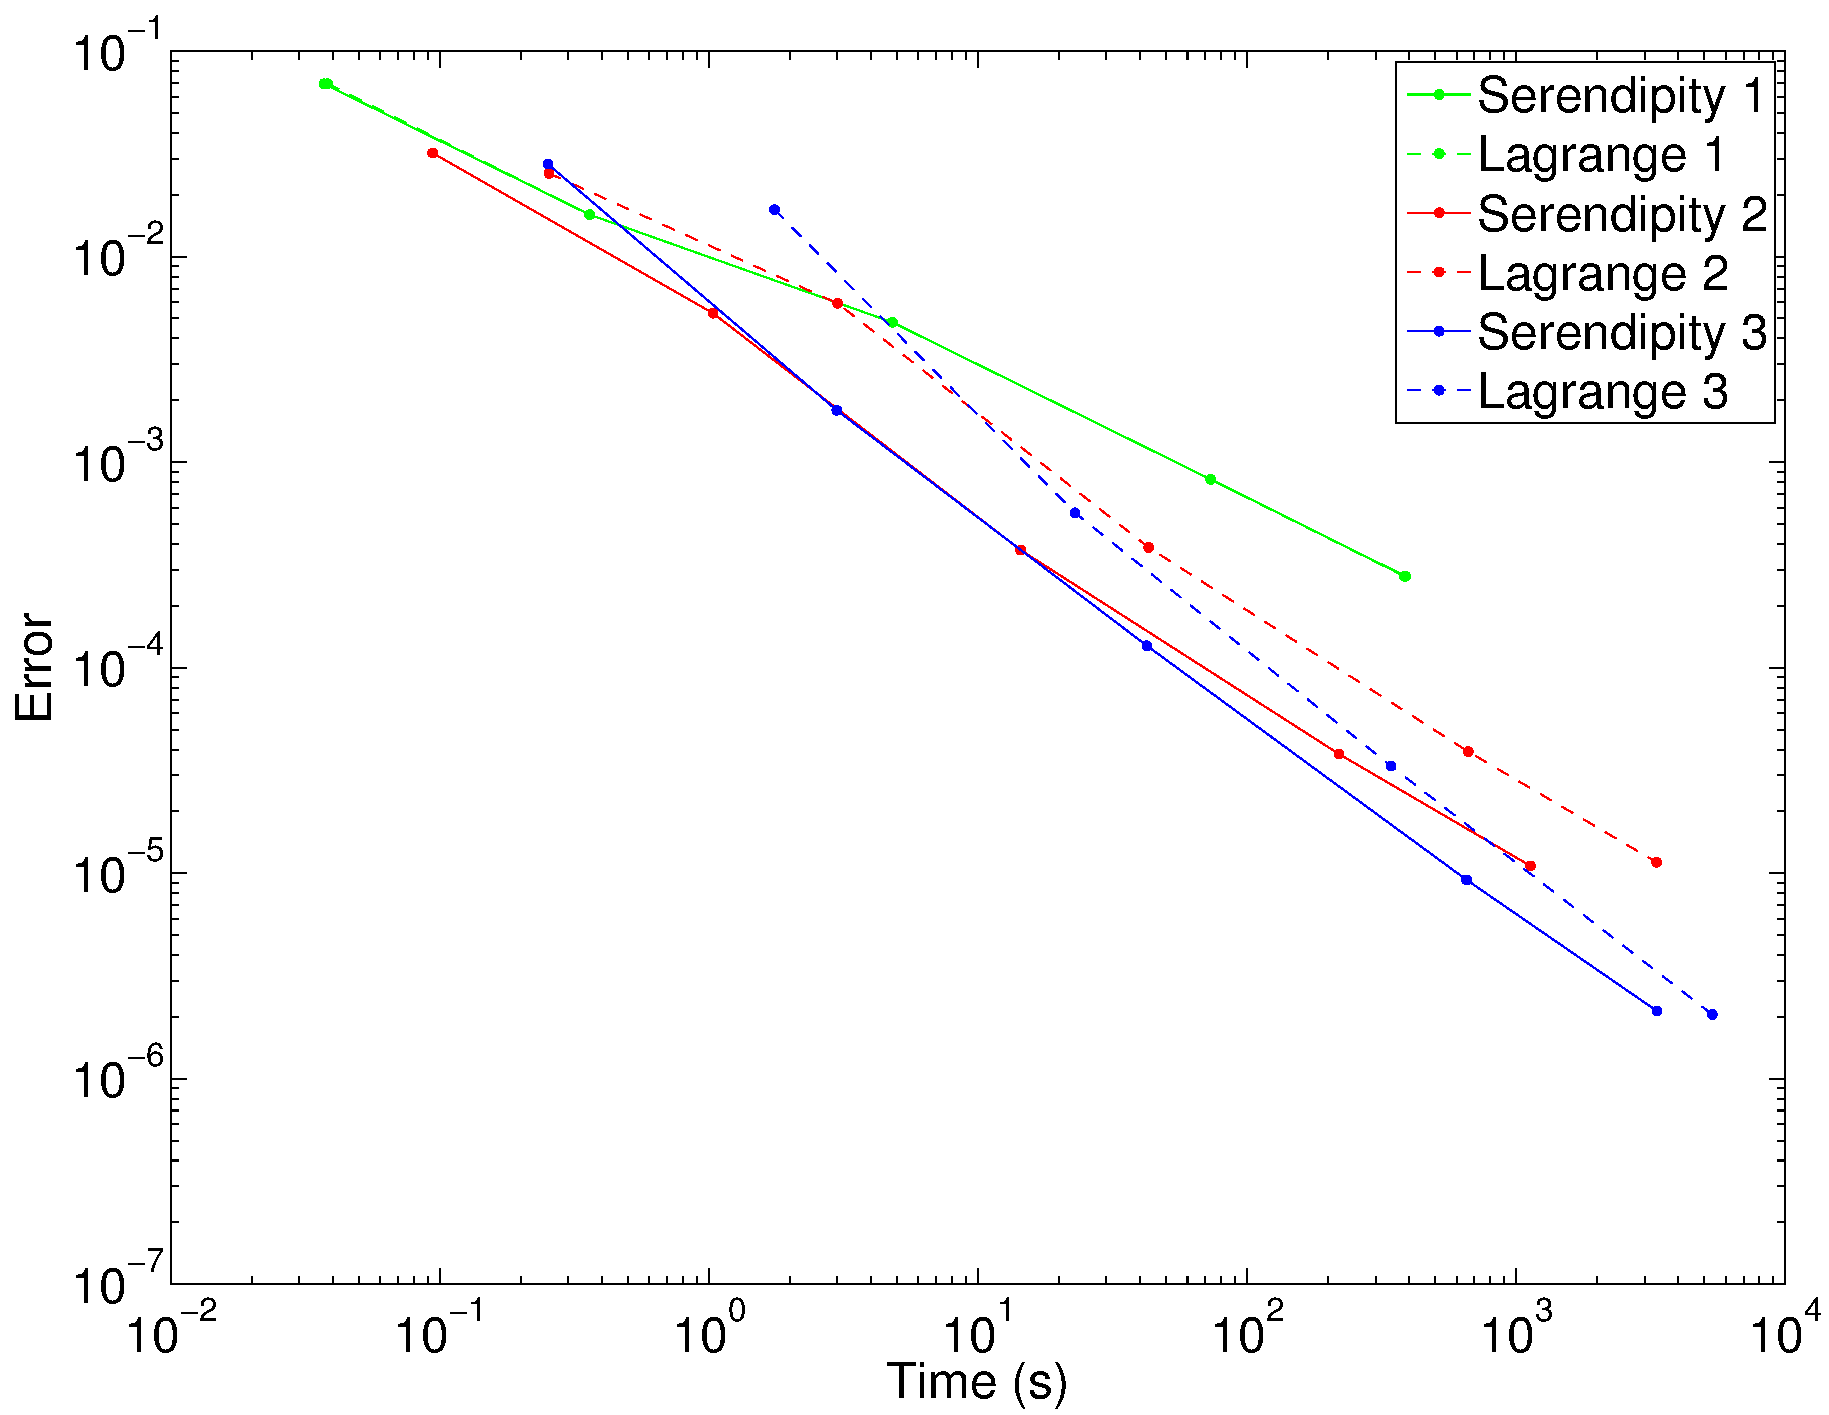
\includegraphics[width=0.8\textwidth]{figures/serendipityConvergence3.pdf}
	\end{figure}
\end{frame}

\begin{frame}
\frametitle{Error vs. Computation Time}
	\begin{figure}
   		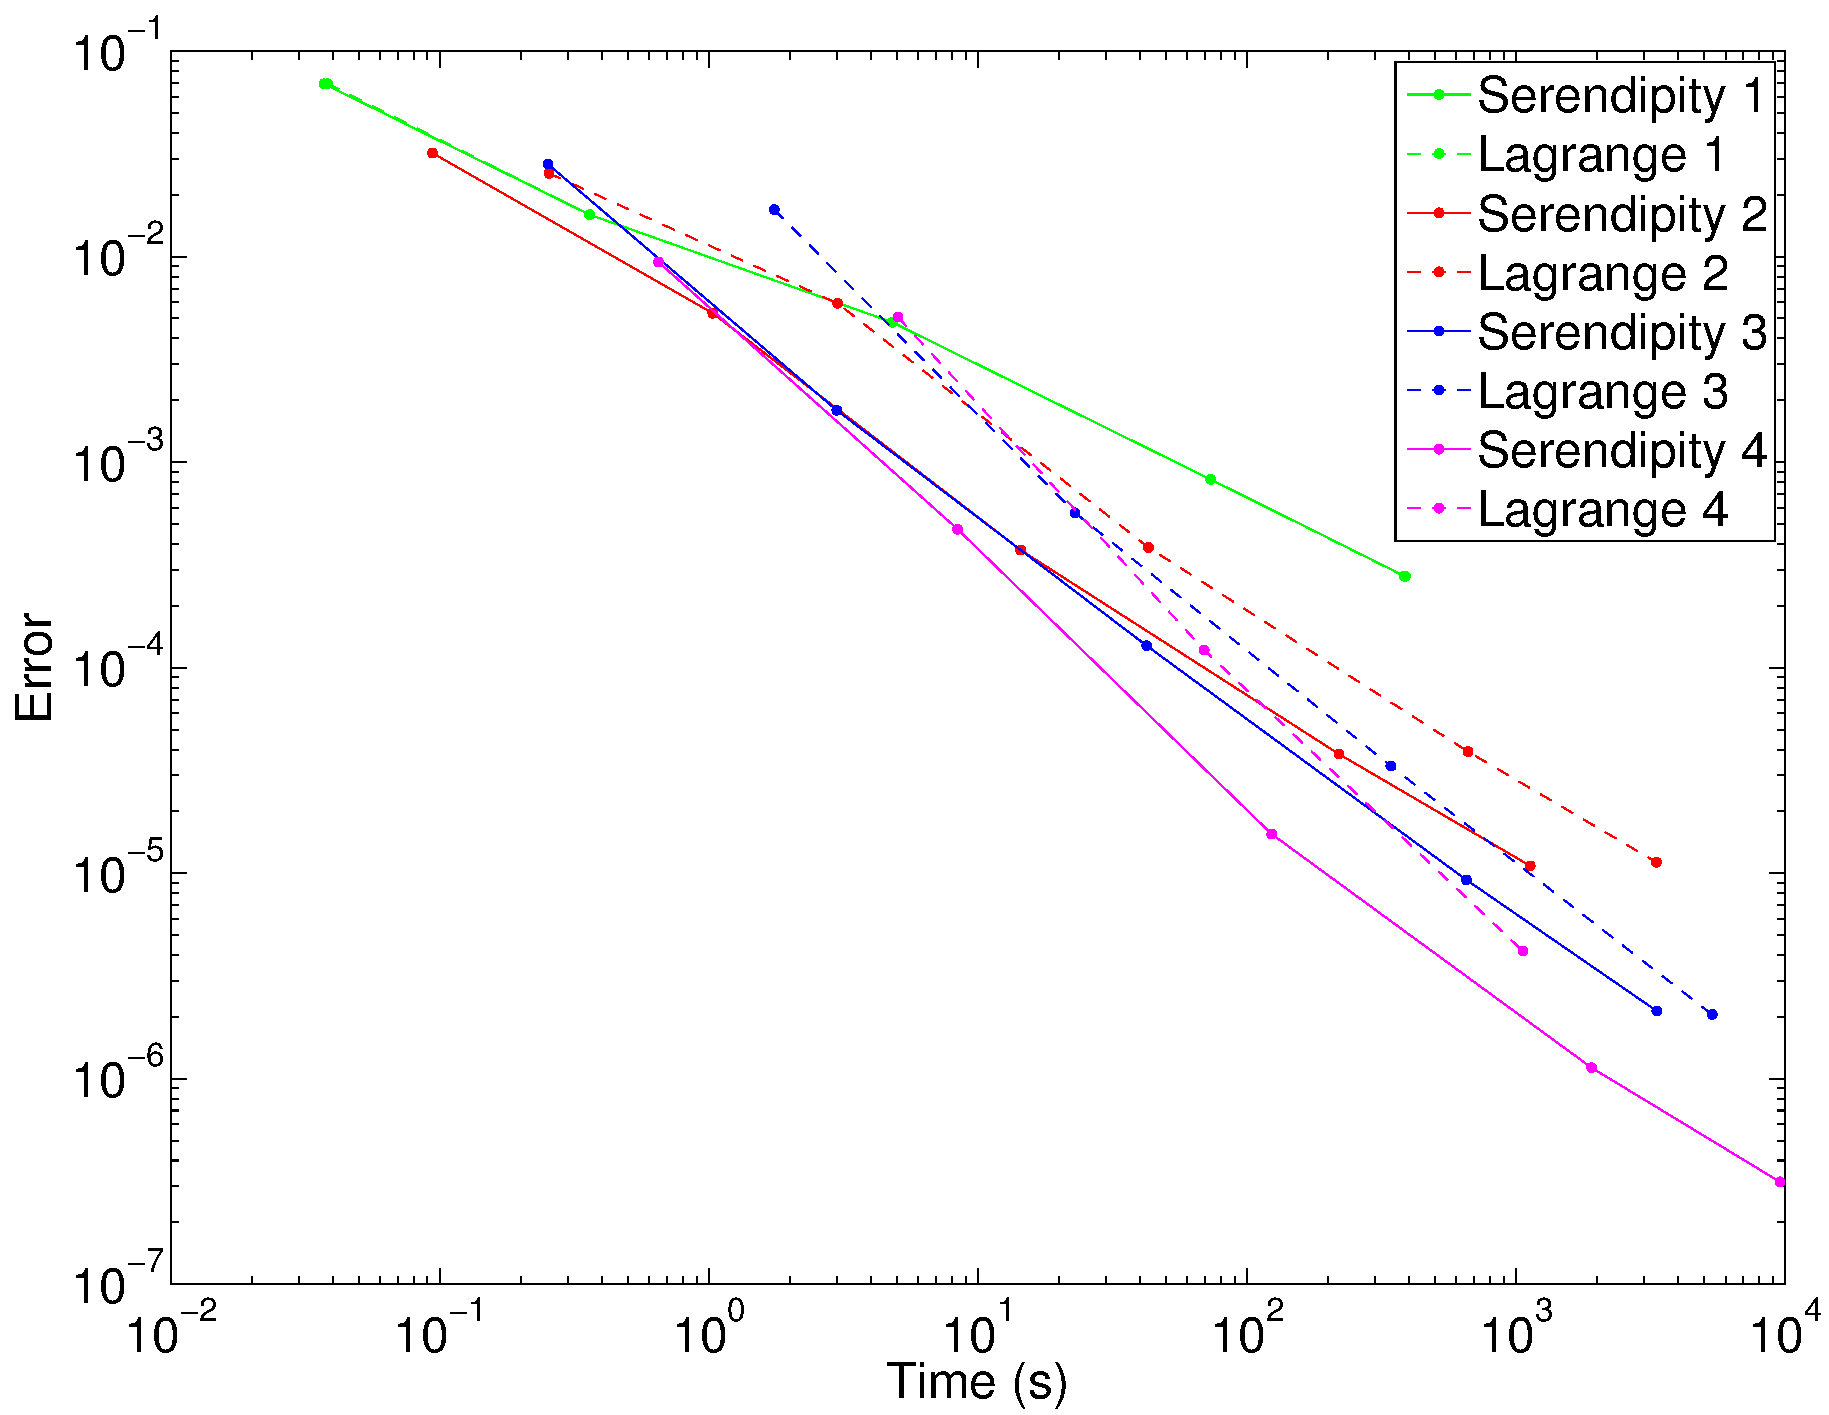
\includegraphics[width=0.8\textwidth]{figures/serendipityConvergence.pdf}
	\end{figure}
\end{frame}

\section{Conclusions}
\begin{frame}
\frametitle{Conclusions}
Initial results indicate that:
\begin{itemize}
	\item Serendipity elements are more efficient than Lagrange elements for obtaining the same level of error
	\item Additional savings in computational time from larger maximum permissible time step for convergence (CFL condition)
\end{itemize}
\end{frame}

\begin{frame}
\frametitle{Future Work}
	\begin{itemize}
		\item Investigate performance of serendipity elements in multi-block structured grids
		\item Use serendipity elements in 1D2V simulations
		\begin{itemize}
			\item Scrape-off layer model
		\end{itemize}
		\item Add full Lenard-Bernstein collision operator
		\item Extend serendipity elements in Gkeyll to 4-D and 5-D
		\item Investigate Maxwellian-weighted basis functions for velocity space discretization
	\end{itemize}
\end{frame}

\begin{frame}
\frametitle{Acknowledgements}
	Thanks to:
	\begin{itemize}
		\item Jeffrey Parker
		\item Chang Liu
	\end{itemize}
	
	Alpha testing:
	\begin{itemize}
		\item Sam Cohen
		\item Allan Reiman
	\end{itemize}
\end{frame}

\begin{frame}
\frametitle{Caveats}
	\begin{itemize}
		\item Reference element in results was mapped to the physical space by scaling each dimension by a constant
		\begin{itemize}
			\item This is an example of an \textbf{affine} map
		\end{itemize}
	\end{itemize}
	\begin{columns}
		\begin{column}{0.7\linewidth}
			\begin{itemize}
				\item Unfortunately, serendipity elements do not attain the same optimal rate of convergence on non-affine meshes%\footfullcite{quadapprox}
			\end{itemize}
		\end{column}
	
		\begin{column}{0.3\linewidth}
			\begin{figure}
				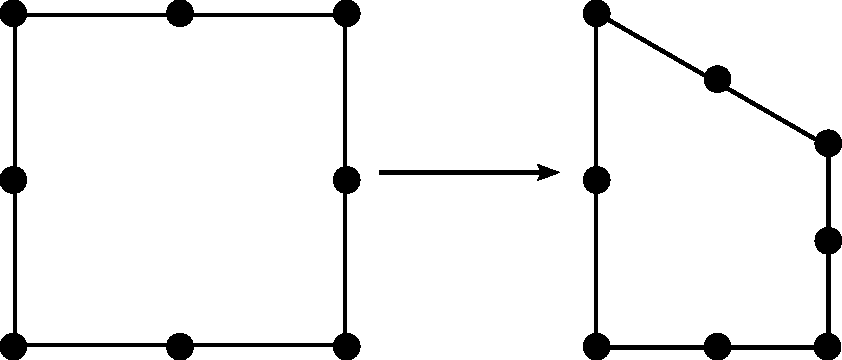
\includegraphics[width=.9\textwidth]{figures/nonaffine.pdf}
			\end{figure}
		\end{column}
	\end{columns}
\begin{itemize}
	
	\item Can avoid this problem by defining basis functions in physical space
\end{itemize}
\end{frame}

\end{document}

